\section{Návrh gest}
\label{chapter:gesta}

V~tejto kapitole popisujeme návrh gest, ktoré
umožnia rozhodcovi zápasenia ovládať aplikáciu
pohybmi zápästia bez nutnosti dotyku displeja
hodiniek. Pri návrhu sme sa inšpirovali reálnymi
gestami rozhodcu na žinenke, aby boli intuitívne
a~rozhodca si nemusel osvojovať novú, nesprávnu
gestikuláciu.

Pri výbere a~definovaní gest sme vychádzali z~oficiálnych
pravidiel Medzinárodnej zápasníckej federácie z~roku~2017
v~slovenskom preklade~\cite{zapasenie_pravidla}, ktoré
presne popisujú, akým spôsobom rozhodca komunikuje svoje
rozhodnutia. Ako doplnkové zdroje sme využili grafický
prehľad gest pre rozhodcov v~zápasení~\cite{wrestling-referee-signals},
ktorý vizuálne zachytáva polohy rúk a~smery pohybu pri
jednotlivých gestách, a~oficiálny inštruktážny videozáznam
Medzinárodnej zápasníckej federácie~\cite{uww-referee-mechanics-video},
ktorý demonštruje správne vykonávanie gest v~praxi.
Kombinácia textového popisu pravidiel, vizuálneho prehľadu
a~videozáznamu nám pomohla pochopiť nielen formálne
požiadavky na gestá, ale aj ich praktickú podobu pri
reálnom zápase.

Navrhnuté gestá rozdeľujeme na \textbf{elementárne}
(Rise Arm, Hand Back, Flick, Hand Down), ktoré
tvoria stavebné prvky, a~\textbf{kompozitné}
(BODOVANIE, PASIVITA, NAPOMENUTIE, TOUCHE), ktoré
sa skladajú z~jedného alebo viacerých elementárnych
gest a~reprezentujú konkrétne akcie rozhodcu počas
zápasu.

\subsection{Princíp rozpoznávania}
\label{subsec:princip-rozpoznavania}

Aplikácia kontinuálne porovnáva aktuálne hodnoty
senzorov s~intervalmi definovanými pre
jednotlivé gestá. Algoritmus pracuje s~kĺzavým časovým
oknom posledných 2~sekúnd a~v~rámci neho hľadá súvislý
úsek dlhý 0{,}2\,ms, počas ktorého sa 100\,\% hodnôt
všetkých troch osí akcelerometra súčasne nachádza
v~definovaných intervaloch daného gesta. Ak takýto
úsek nájde, gesto sa označí ako rozpoznané. Tento
mechanizmus zabraňuje falošným detekciám pri
krátkodobých náhodných pohyboch zápästia a~zároveň
toleruje drobné výkyvy v~rámci 2-sekundového okna --
gesto sa rozpozná aj v~prípade, že hodnoty z~intervalov
nakrátko vystúpia a~následne sa vrátia späť. Tento
časový mechanizmus vysvetľuje aj posun medzi
vstupom hodnôt do hraničných intervalov a~okamihom
detekcie na grafoch v~nasledujúcich podsekciách.

\subsection{Definícia pojmov}
\label{subsection:definicia-pojmov}

Pred podrobným popisom jednotlivých gest definujeme základné pojmy, ktoré budeme v~ďalšom texte
používať. Tieto pojmy označujú elementárne pohyby alebo polohy ruky, z~ktorých sa skladajú
zložitejšie kompozitné gestá.

\begin{description}
  \item[Rise Arm] Pohyb, pri ktorom rozhodca zdvihne ľavú ruku (s~hodinkami) z~neutrálnej polohy
        pri tele do polohy nad hlavou. Slúži ako aktivačné gesto pre
        bodovanie červeného zápasníka. Detailne popísaný v~podsekcii~\ref{subsubsec:rise-arm}.

  \item[Hand Back] Pohyb, pri ktorom rozhodca presunie ľavú ruku (s~hodinkami) za chrbát
        do oblasti krížov, pričom hodinky sú natočené displejom k~chrbtu a~dlaň
        smeruje opačným smerom -- preč od tela. Slúži ako aktivačné gesto pre
        bodovanie modrého zápasníka. Detailne popísaný
        v~podsekcii~\ref{subsubsec:hand-back}.

  \item[Flick] Rýchly rotačný pohyb zápästia proti smeru hodinových ručičiek, zachytený
        gyroskopom. V~aktívnom režime bodovania prideľuje bod zápasníkovi podľa toho, ktoré
        aktivačné gesto bolo predtým vykonané. Detailne popísaný
        v~podsekcii~\ref{subsubsec:flick}.

  \item[Hand Down] Návrat ruky späť do neutrálnej polohy pri tele. Ukončuje akýkoľvek režim
        bodovania a~vracia aplikáciu do režimu čakania. Detailne popísaný
        v~podsekcii~\ref{subsubsec:hand-down}.
\end{description}

Tabuľka~\ref{tab:prehlad-gest} prehľadne zhŕňa všetky navrhnuté gestá.

\begin{table}[H]
  \centering
  \caption{Prehľad navrhnutých gest}
  \label{tab:prehlad-gest}
  \begin{tabularx}{\textwidth}{l l X}
    \toprule
    \textbf{Gesto} & \textbf{Varianty}
                   & \textbf{Správanie aplikácie}              \\
    \midrule
    BODOVANIE      & červený, modrý
                   & Kompozitné gesto: aktivačné gesto
    (Rise Arm pre červeného, Hand Back
    pre modrého) prepne aplikáciu do
    režimu bodovania, Flick prideľuje
    body príslušnému zápasníkovi, Hand
    Down ukončí bodovanie.                                     \\
    \addlinespace
    PASIVITA       & červený, modrý
                   & Zaznamená pasivitu jedného zo zápasníkov. \\
    \addlinespace
    NAPOMENUTIE    & červený, modrý
                   & Automaticky prepne do režimu
    bodovania so zamknutou stranou --
    body idú výhradne súperovi. Bodovanie
    sa opäť ukončí gestom Hand Down.                           \\
    \addlinespace
    TOUCHE & -- & Zaznamená udalosť lopatkového 
            víťazstva ako informačný záznam.                                                  \\
    \bottomrule
  \end{tabularx}
\end{table}

\subsection{Gesto BODOVANIE}

Gesto \uv{Bodovanie} je kompozitné gesto pozostávajúce z~troch po sebe nasledujúcich fáz, ktoré spoločne
umožňujú rozhodcovi prideľovať body jednotlivým zápasníkom. Inšpirovali sme sa reálnym gestom rozhodcu
v~zápasení, kde aktivačné gesto pred gestom \uv{Flick} určuje, ktorému zápasníkovi sa bod udelí. Gesto má dve
alternatívy -- pre červeného a~modrého zápasníka, ktoré sa odlišujú aktivačným gestom v~prvej fáze.

Na obrázku~\ref{fig:bodovanie-flowchart} je znázornený vývojový diagram gesta \uv{Bodovanie}, ktorý
zachytáva spoločnú logiku pre obe alternatívy. Algoritmus začína v~režime čakania, kde čaká na detekciu
jedného z~dvoch aktivačných gest. Po detekcii gesta \uv{Rise Arm} sa prepne do režimu bodovania pre
červeného zápasníka, po detekcii gesta \uv{Hand Back} do režimu bodovania pre modrého zápasníka.
V~oboch prípadoch následne čaká na detekciu flicku proti smeru hodinových ručičiek, ktorý udelí bod
podľa aktívneho režimu. Po prípadnom flicku alebo bez neho algoritmus čaká na gesto \uv{Hand Down},
ktoré ukončí bodovanie a~vráti algoritmus späť do režimu čakania.

\begin{figure}[H]
  \centering
  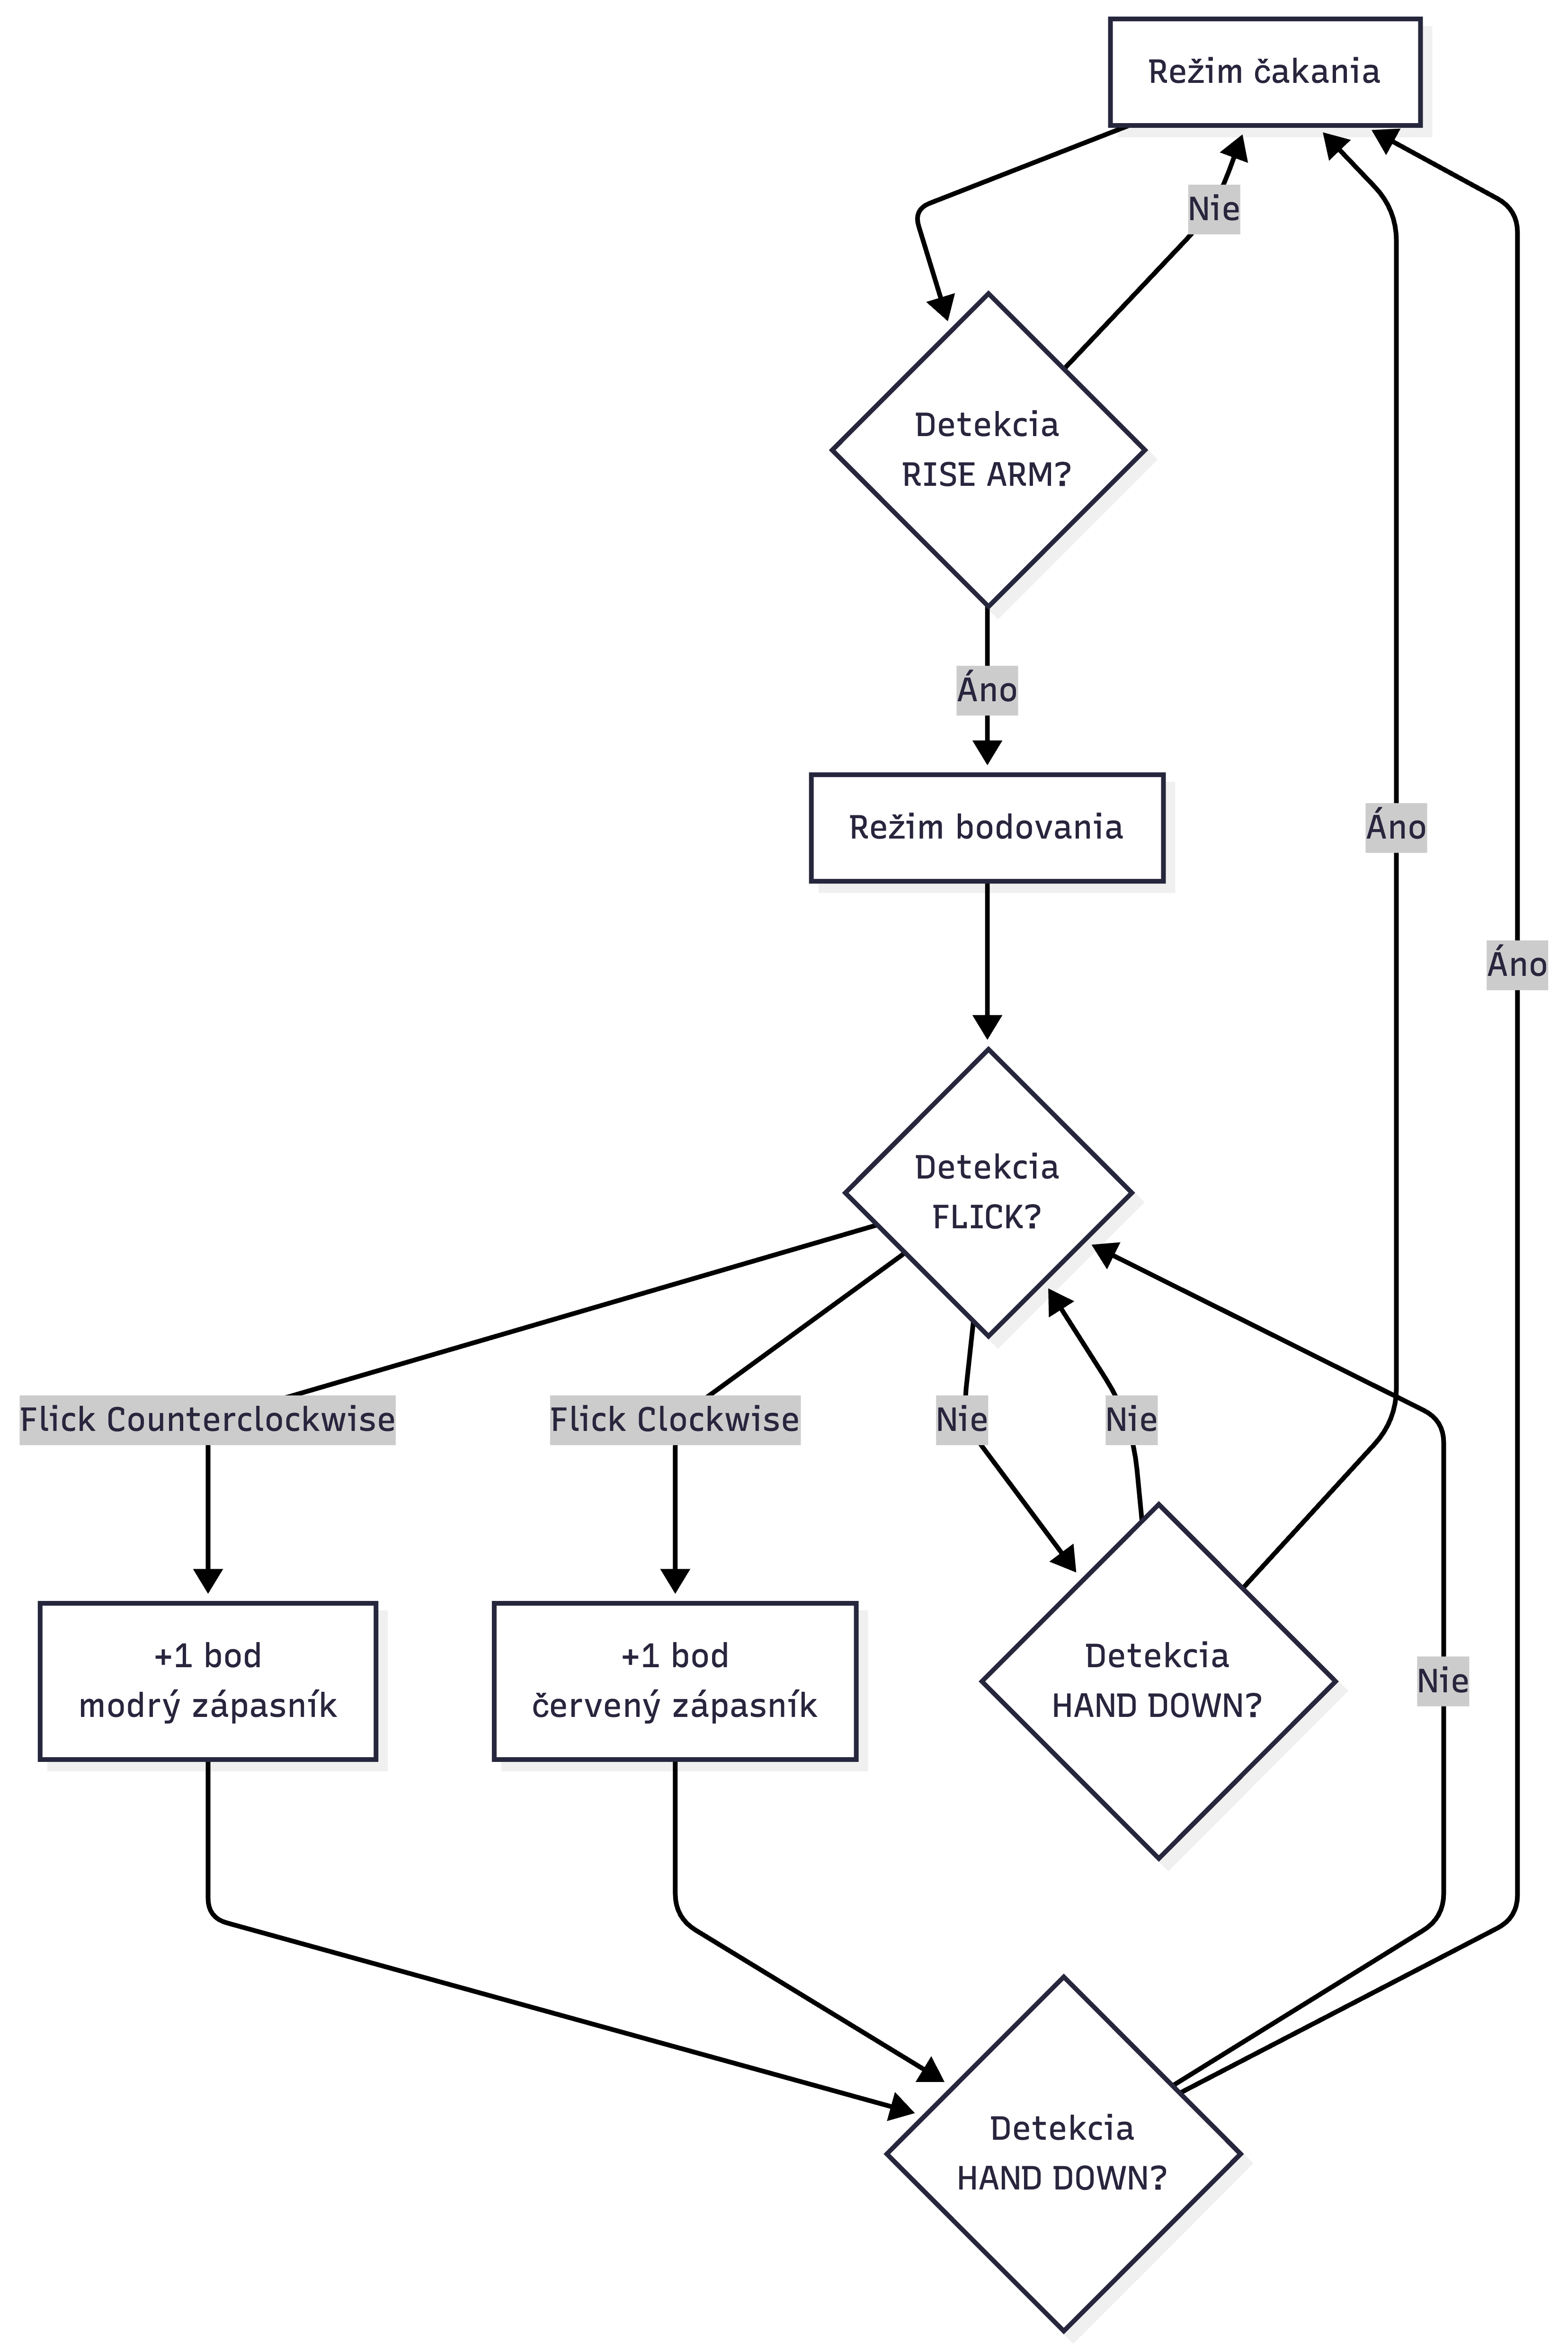
\includegraphics[width=0.6\textwidth]{img/diagrams/flowchart-gesto-bodovanie.png}
  \caption{Vývojový diagram gesta BODOVANIE}
  \label{fig:bodovanie-flowchart}
\end{figure}

\subsubsection{Fáza 1 -- AKTIVÁCIA}

Prvou fázou gesta je aktivácia režimu bodovania pomocou jedného z~dvoch aktivačných gest. Aktivačné
gesto súčasne určuje, ktorému zápasníkovi sa bude bod udeľovať. Aktivačná fáza zároveň slúži ako
ochranný mechanizmus -- gestá \uv{Flick} sú vyhodnocované len vtedy, keď rozhodca vedome vykoná
aktivačné gesto, čím sa predchádza nechcenému pripočítaniu bodov.

\paragraph{Aktivácia pre červeného -- RISE ARM}
\label{subsubsec:rise-arm}
Rozhodca zdvihne ľavú ruku (s~hodinkami) nad hlavu, pričom dlaň smeruje dopredu. Tento pohyb je
detegovaný akcelerometrom inteligentných hodiniek, ktorý zaznamenáva zmenu orientácie zápästia.
Po rozpoznaní gesta \uv{Rise Arm} sa aplikácia prepne do režimu bodovania pre červeného zápasníka.

\begin{figure}[H]
  \centering
  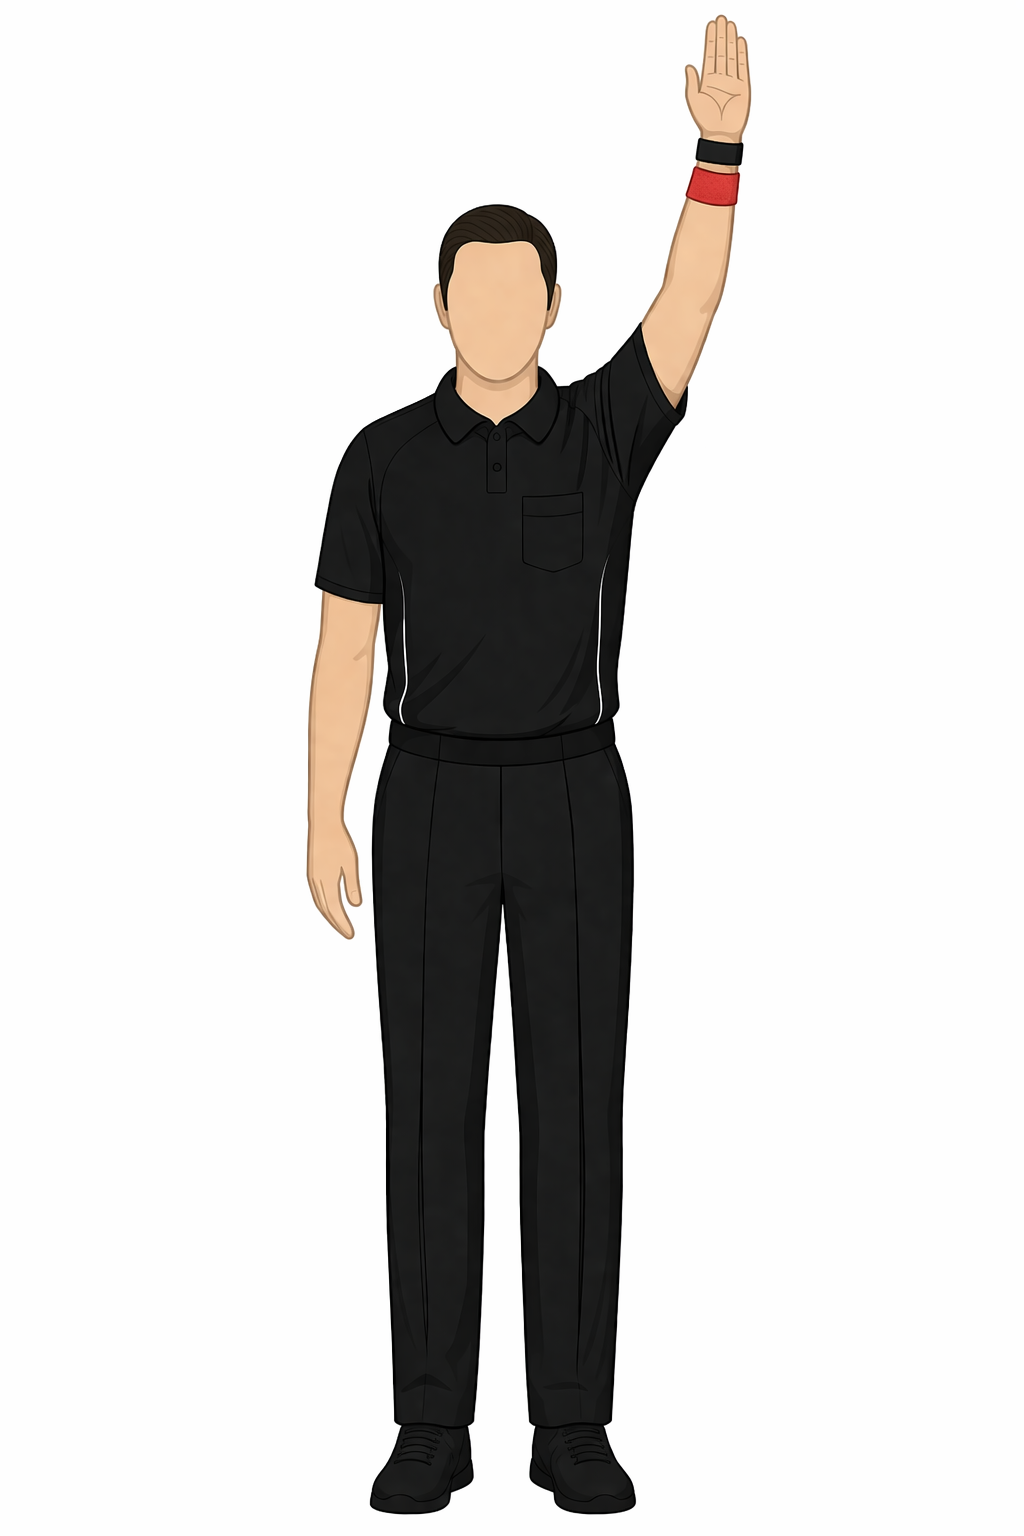
\includegraphics[width=0.4\textwidth]{img/gesture-img/obrazok-gesto-rise-arm.png}
  \caption{Poloha ruky pri geste \uv{Rise Arm}}
  \label{fig:gesto-rise-arm}
\end{figure}

Na obrázku~\ref{fig:gesto-rise-arm} je znázornená poloha ruky rozhodcu pri geste \uv{Rise Arm}. Ľavá
ruka s~hodinkami a~červenou manžetou je zdvihnutá nad hlavu a~zároveň dlaň smeruje dopredu. Táto
poloha zodpovedá reálnemu gestu rozhodcu na žinenke, ktorým oznamuje začiatok bodovania pre
červeného zápasníka ostatným členom rozhodcovského tímu.

\begin{figure}[H]
  \centering
  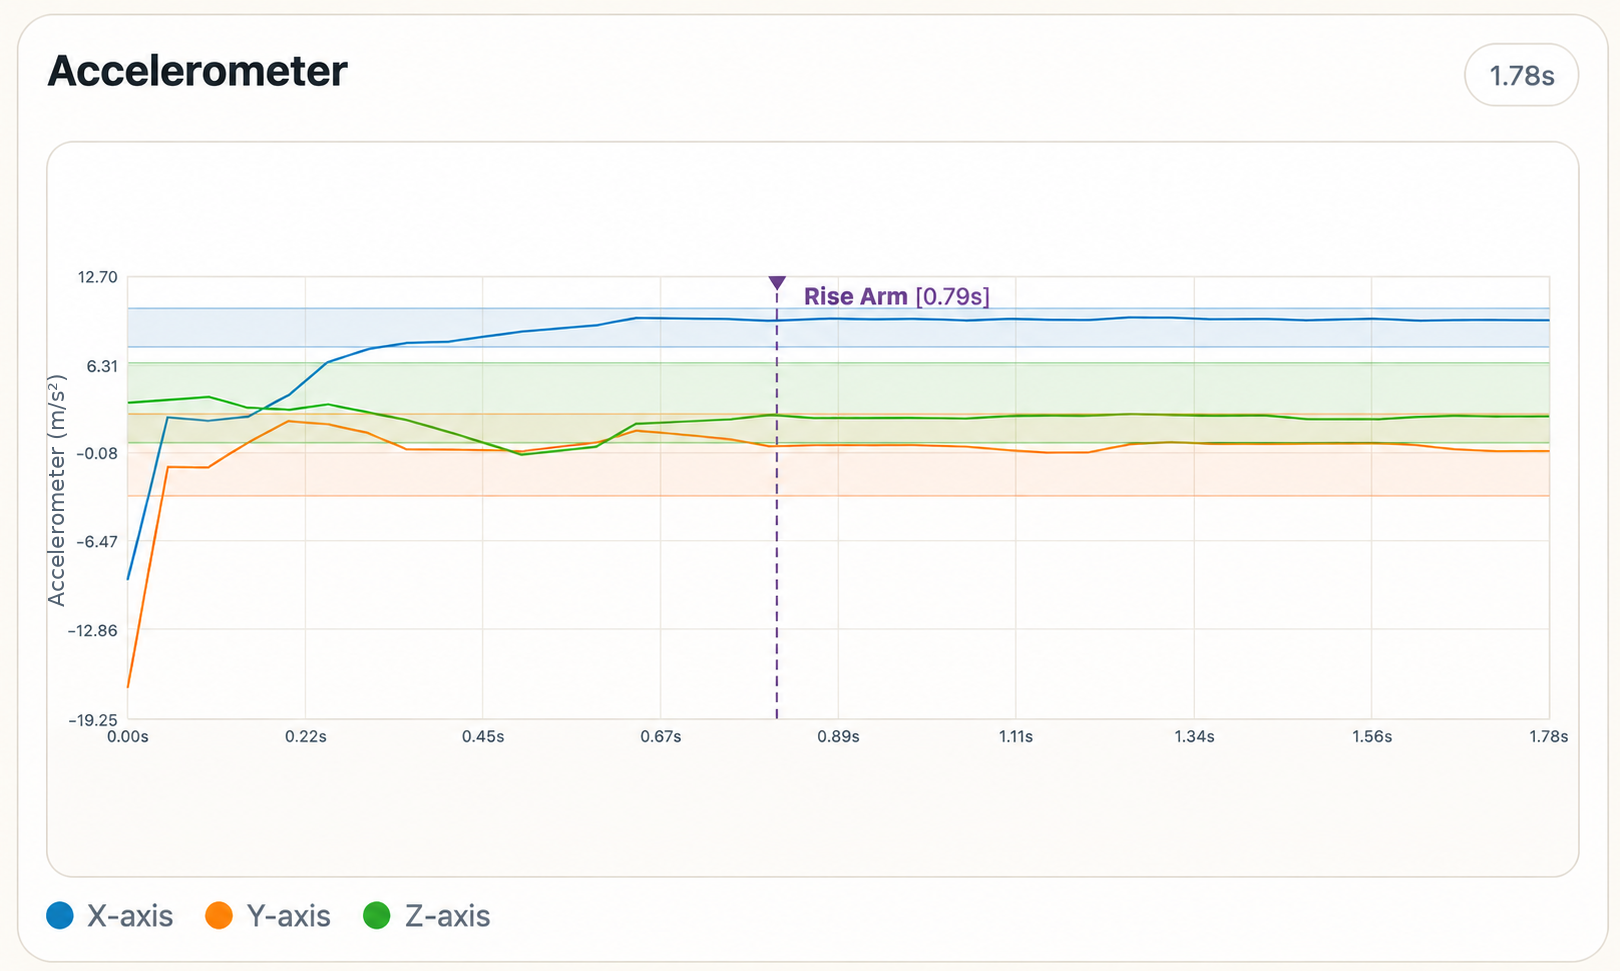
\includegraphics[width=0.9\textwidth]{img/gesture-flow/flow-gesto-rise-arm.png}
  \caption{Príklad priebehu akcelerometrických dát počas gesta \uv{Rise Arm}.}
  \label{fig:subgesture-hand-up}
\end{figure}

Na obrázku~\ref{fig:subgesture-hand-up} je zobrazený priebeh akcelerometrických dát počas vykonania
gesta \uv{Rise Arm} a označený bod, kedy dochádza k~detekcii tohto gesta.

Interval hodnôt pre rozpoznanie gesta \uv{Rise Arm}, kde $a_x$, $a_y$ a~$a_z$ označujú hodnoty
zrýchlenia na príslušných osiach akcelerometra:

\begin{itemize}
  \item \colorbox{xaxis!20}{$\handUpAxMin \leq a_x \leq \handUpAxMax \;\text{m/s}^2$}
  \item \colorbox{yaxis!20}{$\handUpAyMin \leq a_y \leq \handUpAyMax \;\text{m/s}^2$}
  \item \colorbox{zaxis!20}{$\handUpAzMin \leq a_z \leq \handUpAzMax \;\text{m/s}^2$}
\end{itemize}

\paragraph{Aktivácia pre modrého -- HAND BACK}
\label{subsubsec:hand-back}

Rozhodca presunie ľavú ruku (s~hodinkami) za chrbát do oblasti krížov,
pričom zápästie je rotované tak, že displej hodiniek je natočený smerom
k~chrbtu a~dlaň smeruje preč od tela. Po rozpoznaní
gesta \uv{Hand Back} sa aplikácia prepne do režimu bodovania pre modrého zápasníka.

\begin{figure}[H]
  \centering
  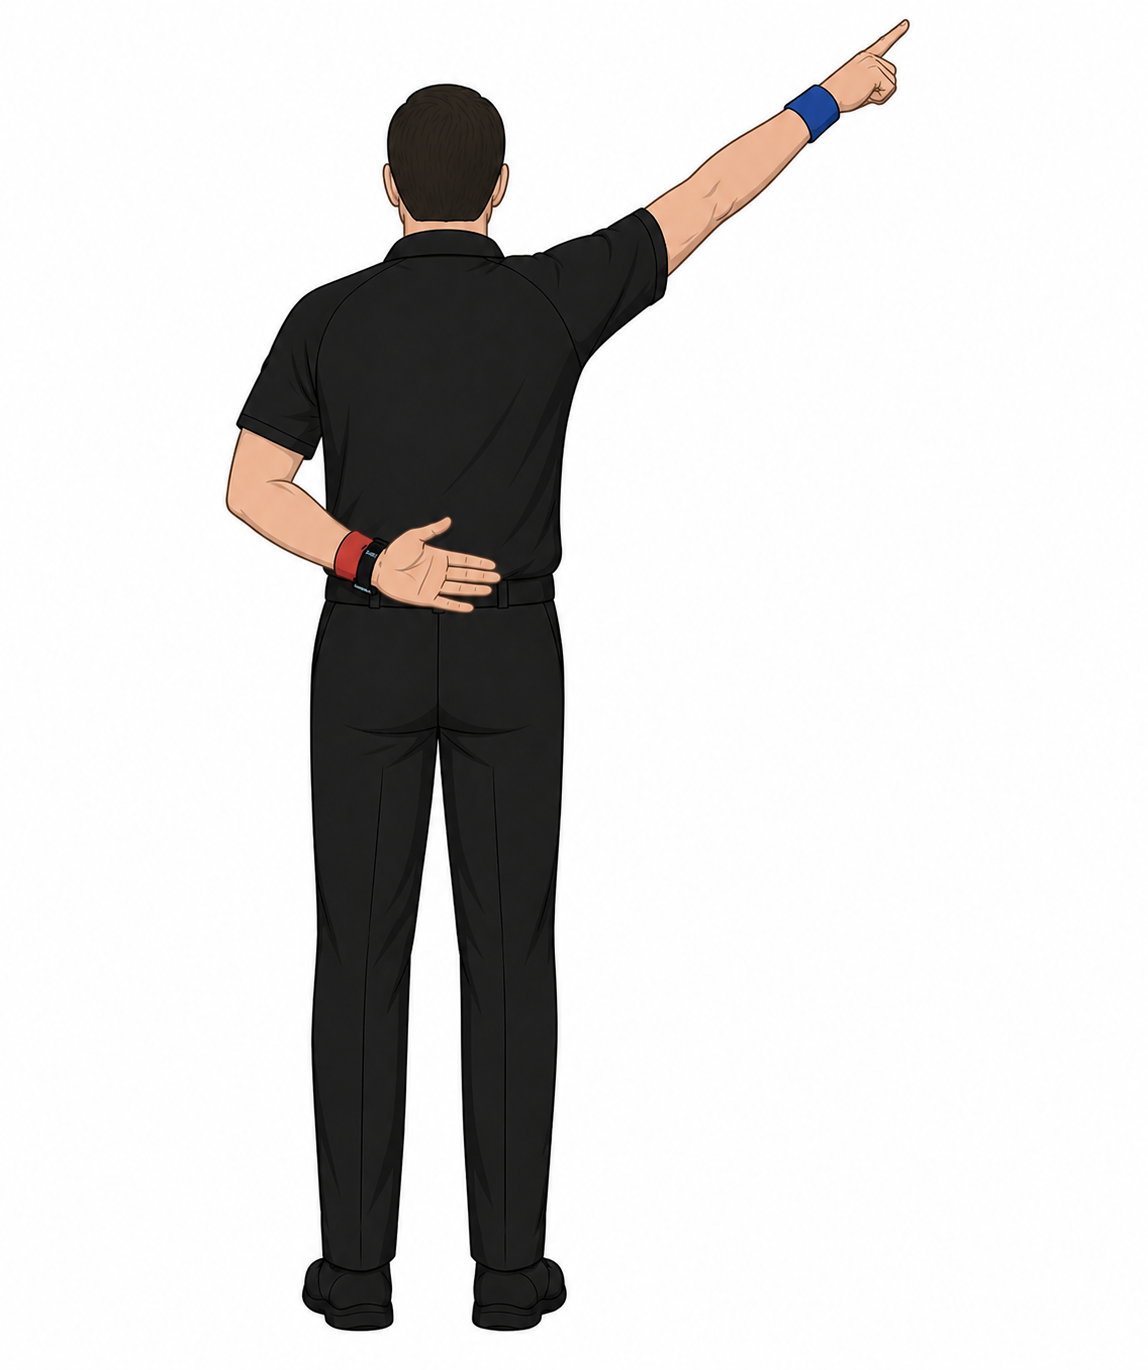
\includegraphics[width=0.4\textwidth]{img/gesture-img/obrazok-gesto-hand-back.png}
  \caption{Poloha ruky pri geste \uv{Hand Back}}
  \label{fig:gesto-hand-back}
\end{figure}

\begin{figure}[H]
  \centering
  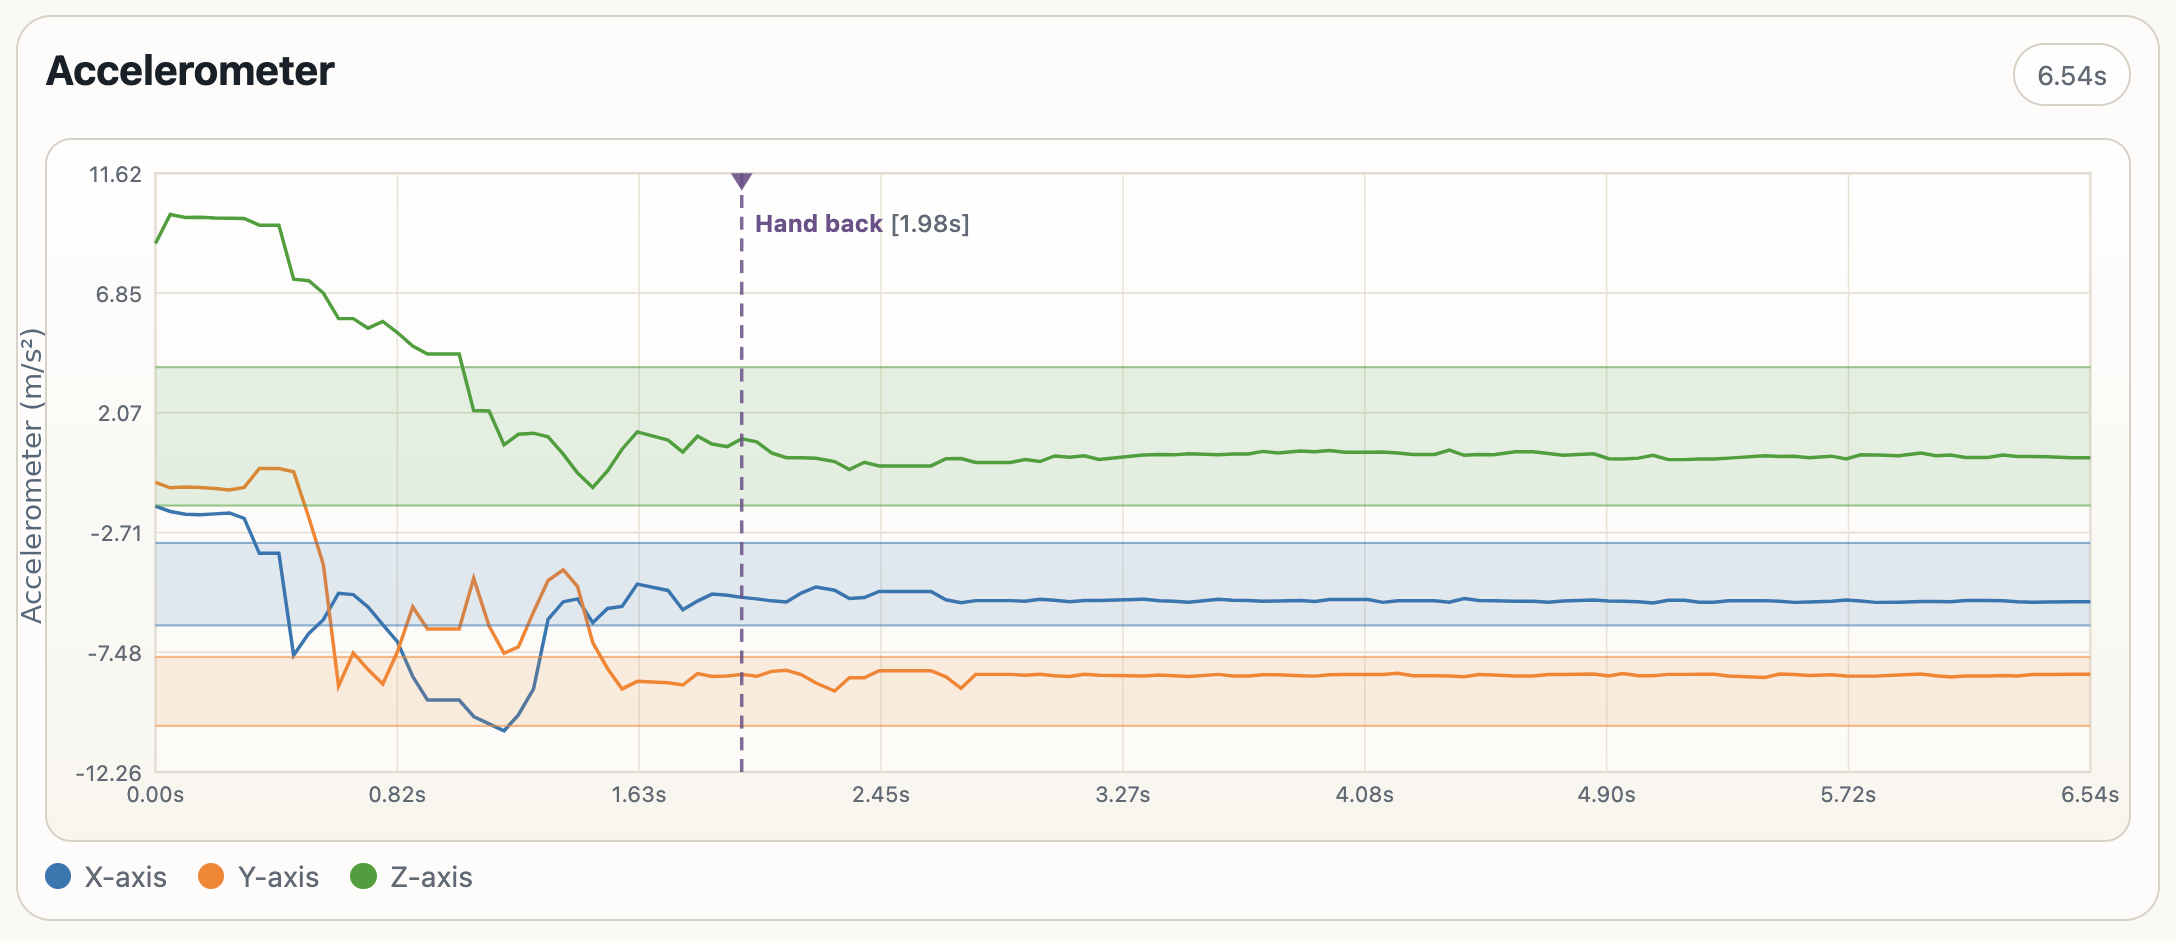
\includegraphics[width=0.9\textwidth]{img/gesture-flow/flow-gesto-hand-back.png}
  \caption{Príklad priebehu akcelerometrických dát počas gesta \uv{Hand Back}.}
  \label{fig:subgesture-hand-back}
\end{figure}

Na obrázku~\ref{fig:subgesture-hand-back} je zobrazený priebeh akcelerometrických
dát počas vykonania gesta \uv{Hand Back} a~označený bod, kedy dochádza
k~detekcii tohto gesta.

\noindent
\textbf{Interval hodnôt:}

\begin{itemize}
  \item \colorbox{xaxis!20}{$\handBackAxMin \leq a_x \leq \handBackAxMax \;\text{m/s}^2$}
  \item \colorbox{yaxis!20}{$\handBackAyMin \leq a_y \leq \handBackAyMax \;\text{m/s}^2$}
  \item \colorbox{zaxis!20}{$\handBackAzMin \leq a_z \leq \handBackAzMax \;\text{m/s}^2$}
\end{itemize}

Ak sa hodnoty všetkých troch osí súčasne nachádzajú v~rámci uvedených rozsahov pre dané aktivačné
gesto, aplikácia sa prepne do príslušného režimu bodovania, v~ktorom sú následne vyhodnocované
gestá \uv{Flick}.

\subsubsection{Fáza 2 -- FLICK}
\label{subsubsec:flick}

Po aktivácii režimu bodovania rozhodca vykoná rýchly rotačný pohyb zápästia proti smeru hodinových
ručičiek, ktorý je zachytený gyroskopickým senzorom hodiniek. Bod sa pridelí podľa aktívneho režimu
nastaveného v~prvej fáze:

\begin{itemize}
  \item Ak bol režim aktivovaný gestom \uv{Rise Arm}, flick pridelí bod \textbf{červenému} zápasníkovi.
  \item Ak bol režim aktivovaný gestom \uv{Hand Back}, flick pridelí bod \textbf{modrému} zápasníkovi.
\end{itemize}

Dáta z~gyroskopu sú prenášané do telefónu, kde algoritmus vyhodnocuje uhlovú rýchlosť rotácie na osi
$g_x$, kde $g_x$ označuje hodnotu uhlovej rýchlosti na príslušnej osi gyroskopického senzora
v~jednotkách stupňov za sekundu ($^\circ$/s). Na základe analýzy nameraných gyroskopických dát bola
stanovená nasledovná prahová hodnota pre rozpoznanie flicku:

\begin{itemize}
  \item \colorbox{xaxis!20}{$g_x < \flckBlueThreshold \;^\circ\text{/s}$} -- rotácia proti smeru
        hodinových ručičiek prekročí prahovú hodnotu $\flckBlueThreshold\,^\circ\text{/s}$.
\end{itemize}

\begin{figure}[H]
  \centering
  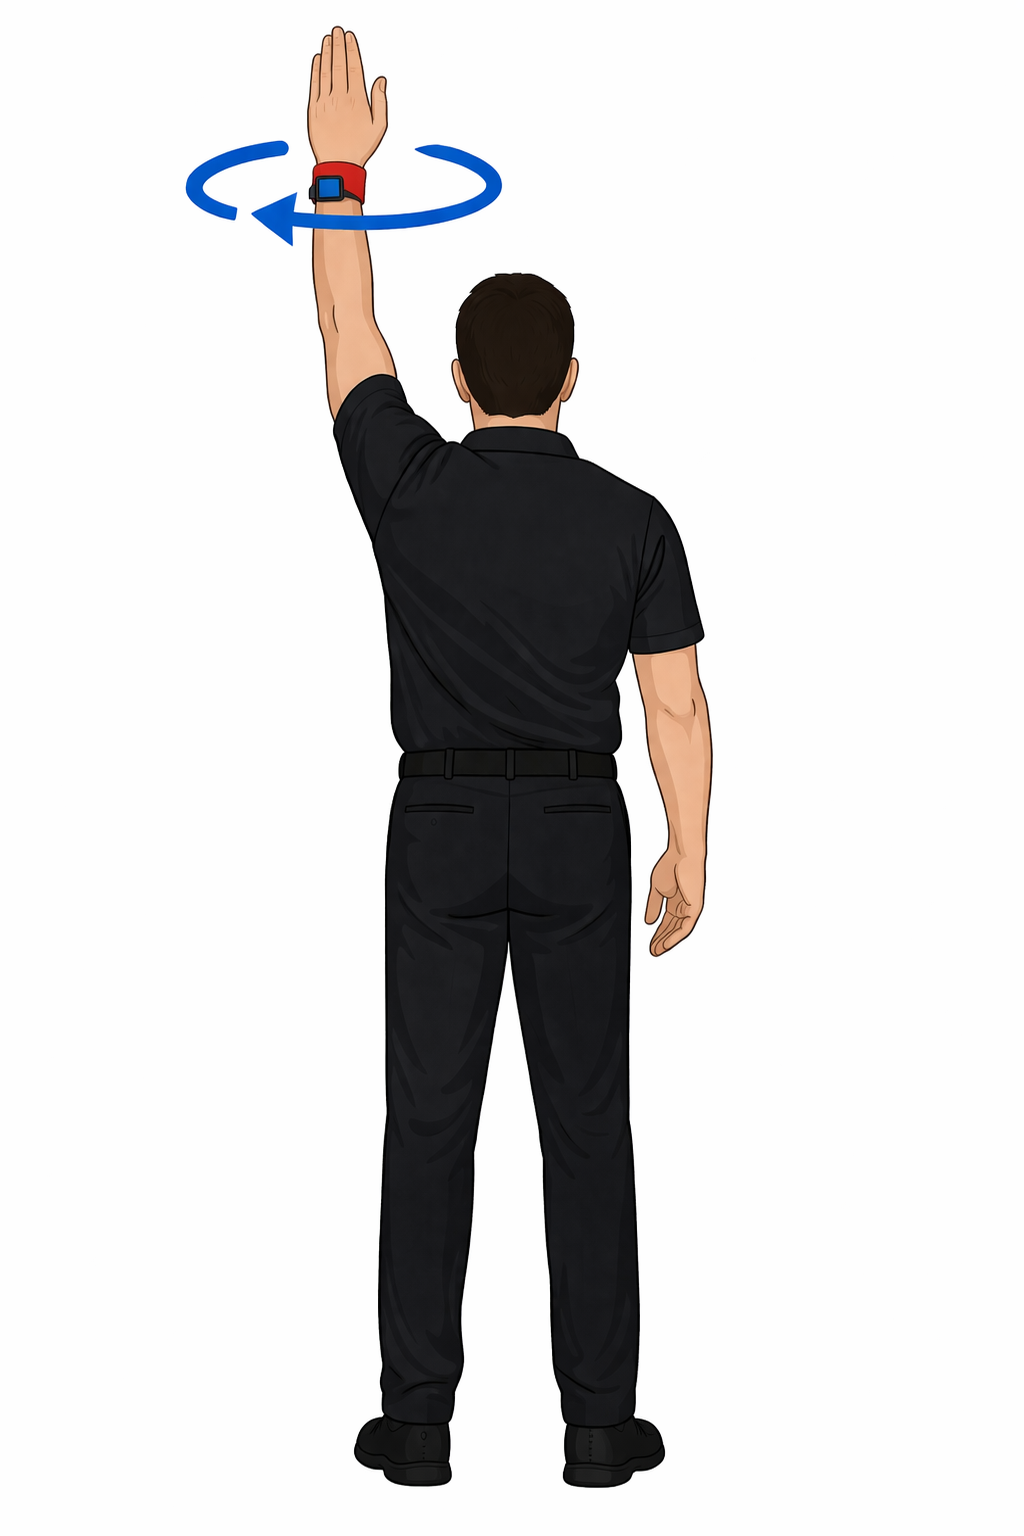
\includegraphics[width=0.40\textwidth]{img/gesture-img/obrazok-gesto-flick-counterclockwise.png}
  \caption{Pohyb zápästia pri geste \uv{Flick}}
  \label{fig:gesto-flick-ccw}
\end{figure}

Na obrázku~\ref{fig:gesto-flick-ccw} je znázornený pohyb zápästia pri geste \uv{Flick}.
Rozhodca vykoná rýchlu rotáciu zápästia proti smeru hodinových ručičiek, čo je na obrázku znázornené
modrou šípkou. Tento pohyb je zachytený gyroskopom na osi $g_x$ ako výrazný záporný špičkový výkyv.

\begin{figure}[H]
  \centering
  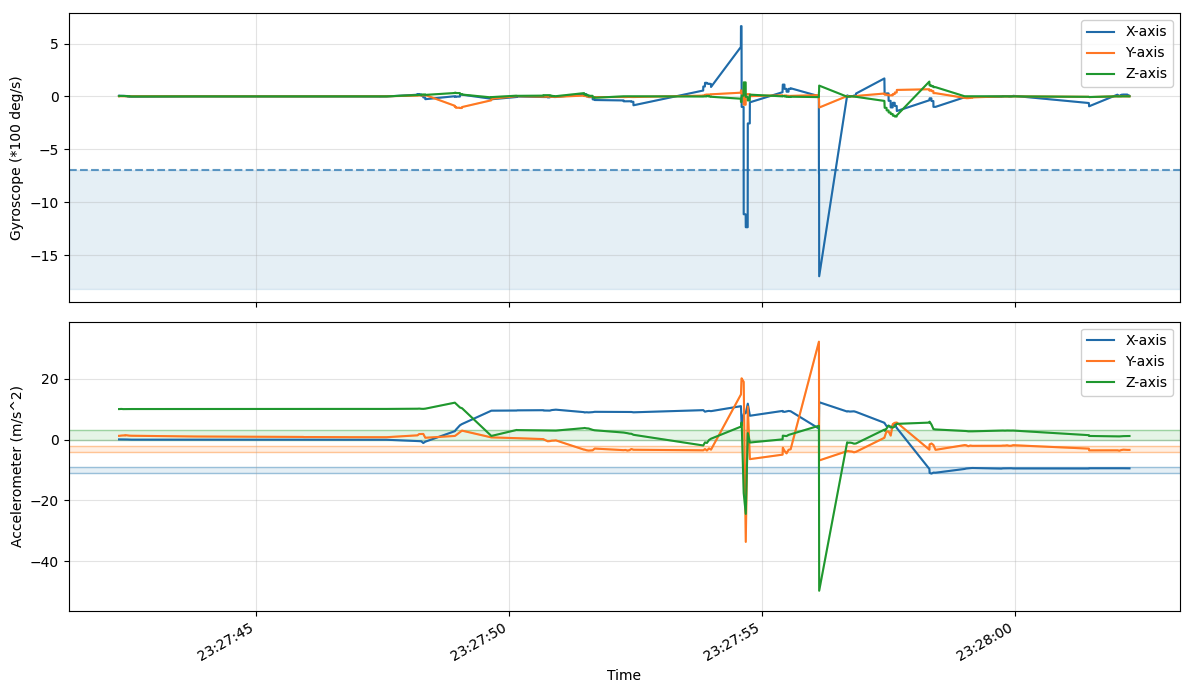
\includegraphics[width=0.9\textwidth]{img/gesture-flow/flow-gesto-flick-counterclockwise.png}
  \caption{Príklad priebehu gyroskopických a~akcelerometrických dát počas gesta
    \uv{Flick}.}
  \label{fig:subgesture-flick-ccw}
\end{figure}

Na obrázku~\ref{fig:subgesture-flick-ccw} je zobrazený priebeh senzorových dát počas vykonania gesta
\uv{Flick}. V~hornej časti grafu, ktorá zachytáva gyroskopické dáta, je viditeľný
výrazný záporný špičkový výkyv na osi $g_x$ (modrá), ktorý dosahuje hodnotu približne
$-1600\,^\circ\text{/s}$, čo výrazne prekračuje stanovenú prahovú hodnotu
$\flckBlueThreshold\,^\circ\text{/s}$. Práve tento krátkodobý, ale intenzívny výkyv je kľúčovým
signálom, na základe ktorého algoritmus rozpozná flick a~pridelí bod podľa aktívneho režimu.
V~spodnej časti grafu sú zobrazené akcelerometrické dáta, na ktorých je viditeľný sprievodný otras
spôsobený rýchlym pohybom zápästia.

Rozhodca môže v~rámci jednej aktivácie vykonať aj viacero po sebe nasledujúcich gest \uv{Flick},
pokiaľ neukončí fázu bodovania gestom \uv{Hand Down}. Tým je umožnené prideliť viacero bodov bez
nutnosti opakovane vykonávať aktivačné gesto.

\subsubsection{Fáza 3 -- HAND DOWN}
\label{subsubsec:hand-down}

Poslednou fázou je návrat ruky do neutrálnej polohy pri tele. Akcelerometer deteguje návrat
zápästia do neutrálnej orientácie, čo signalizuje ukončenie procesu bodovania. Po rozpoznaní gesta
\uv{Hand Down} sa aplikácia prepne späť do režimu čakania, v~ktorom je gesto \uv{Flick} ignorované.
Tým je zabezpečené, že bežné pohyby ruky rozhodcu počas zápasu nevedú k~neúmyselnému prideľovaniu bodov.

\begin{figure}[H]
  \centering
  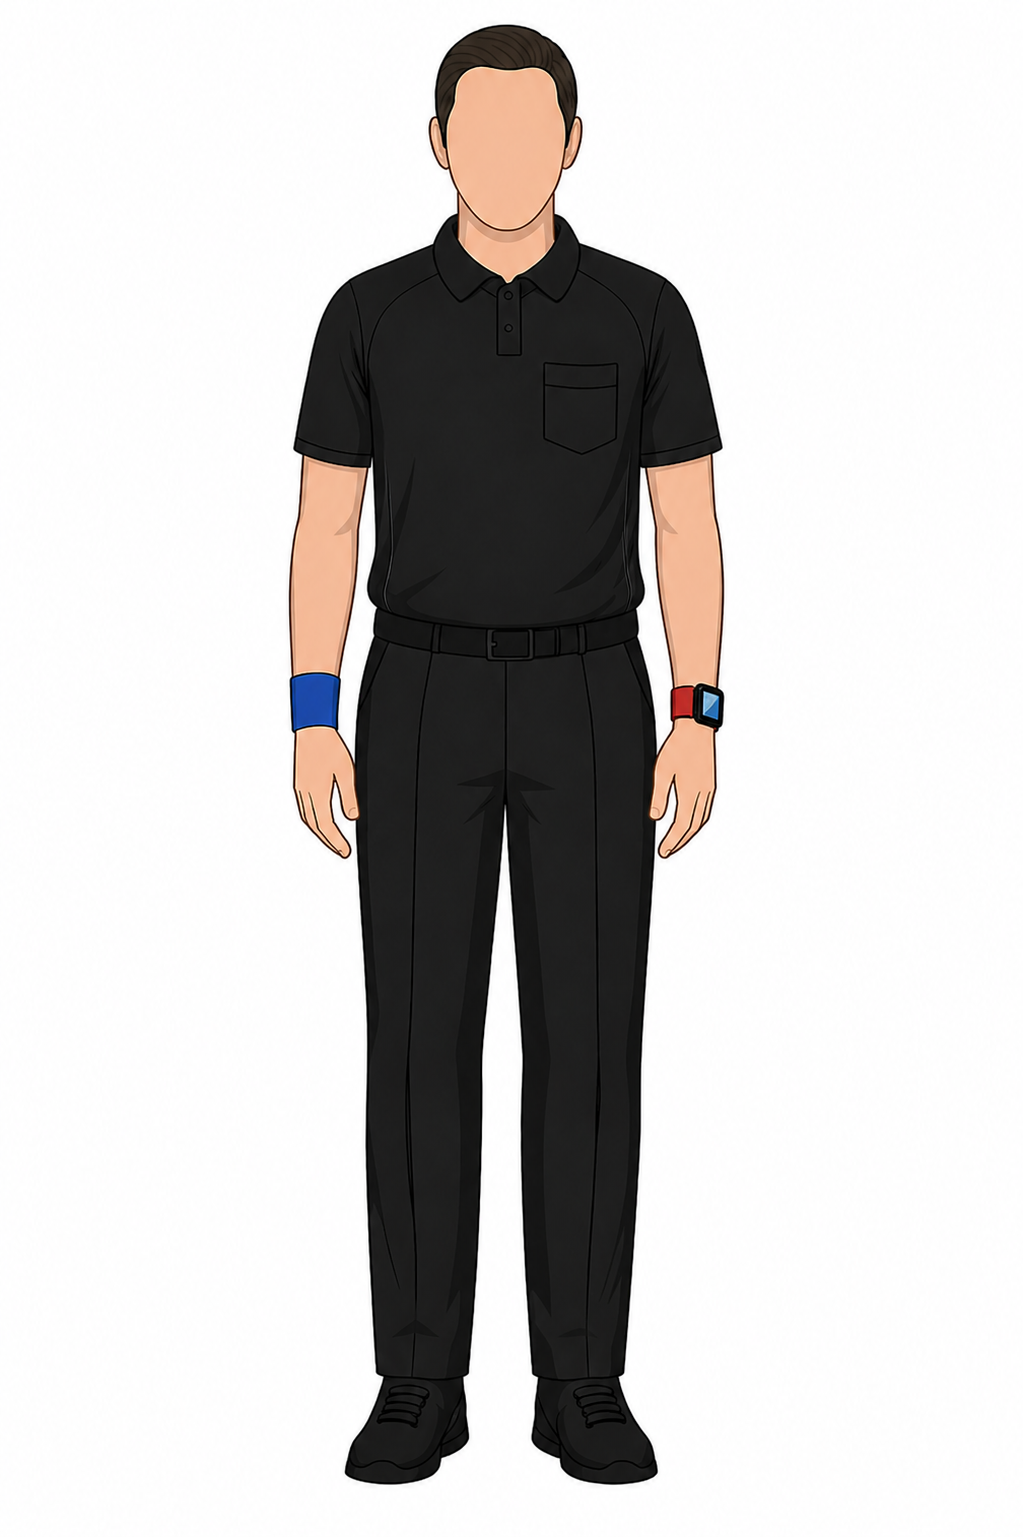
\includegraphics[width=0.4\textwidth]{img/gesture-img/obrazok-gesto-hand-down.png}
  \caption{Poloha ruky pri geste \uv{Hand Down}}
  \label{fig:gesto-hand-down}
\end{figure}

\begin{figure}[H]
  \centering
  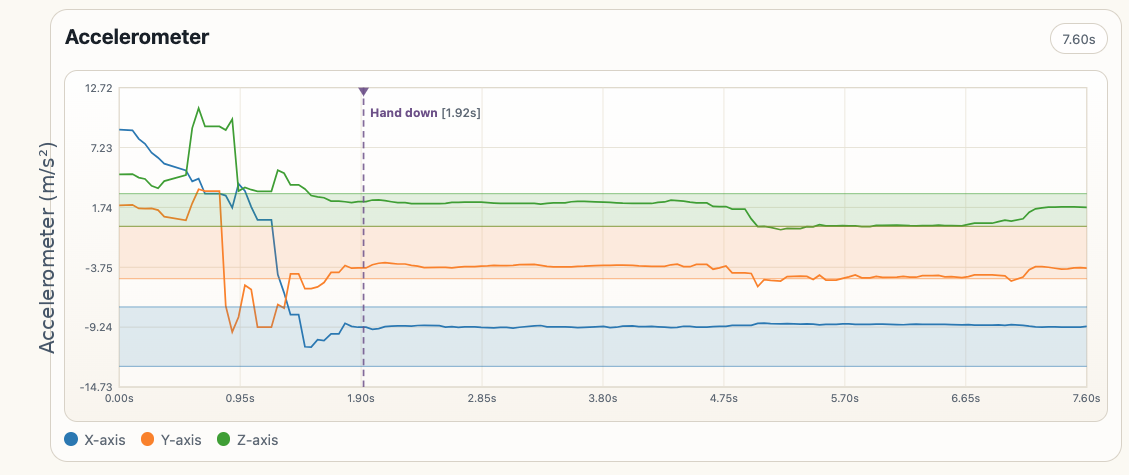
\includegraphics[width=0.9\textwidth]{img/gesture-flow/flow-gesto-hand-down.png}
  \caption{Príklad priebehu akcelerometrických dát počas gesta \uv{Hand Down}.}
  \label{fig:subgesture-hand-down}
\end{figure}

Na obrázku~\ref{fig:subgesture-hand-down} je zobrazený priebeh akcelerometrických dát počas
vykonania gesta \uv{Hand Down}. Z~grafu je zrejmé, že hodnoty jednotlivých osí sa po návrate ruky
ustália v~rámci definovaných intervalov hodnôt.

Interval hodnôt pre rozpoznanie gesta \uv{Hand Down}:

\begin{itemize}
  \item \colorbox{xaxis!20}{$\handDownAxMin \leq a_x \leq \handDownAxMax \;\text{m/s}^2$}
  \item \colorbox{yaxis!20}{$\handDownAyMin \leq a_y \leq \handDownAyMax \;\text{m/s}^2$}
  \item \colorbox{zaxis!20}{$\handDownAzMin \leq a_z \leq \handDownAzMax \;\text{m/s}^2$}
\end{itemize}

Ak sa hodnoty všetkých troch osí súčasne nachádzajú v~rámci uvedených rozsahov, dôjde k~úspešnému
rozpoznaniu gesta \uv{Hand Down} a~aplikácia sa prepne späť do režimu čakania.

\subsubsection{Priebeh celého gesta BODOVANIE}

Pre lepšiu predstavu o~tom, ako jednotlivé fázy gesta \uv{Bodovanie} nadväzujú na seba v~reálnom
čase, uvádzame na obrázku~\ref{fig:bodovanie-priebeh} priebeh senzorových dát počas vykonania
celého kompozitného gesta vrátane všetkých troch fáz.

\begin{figure}[H]
  \centering
  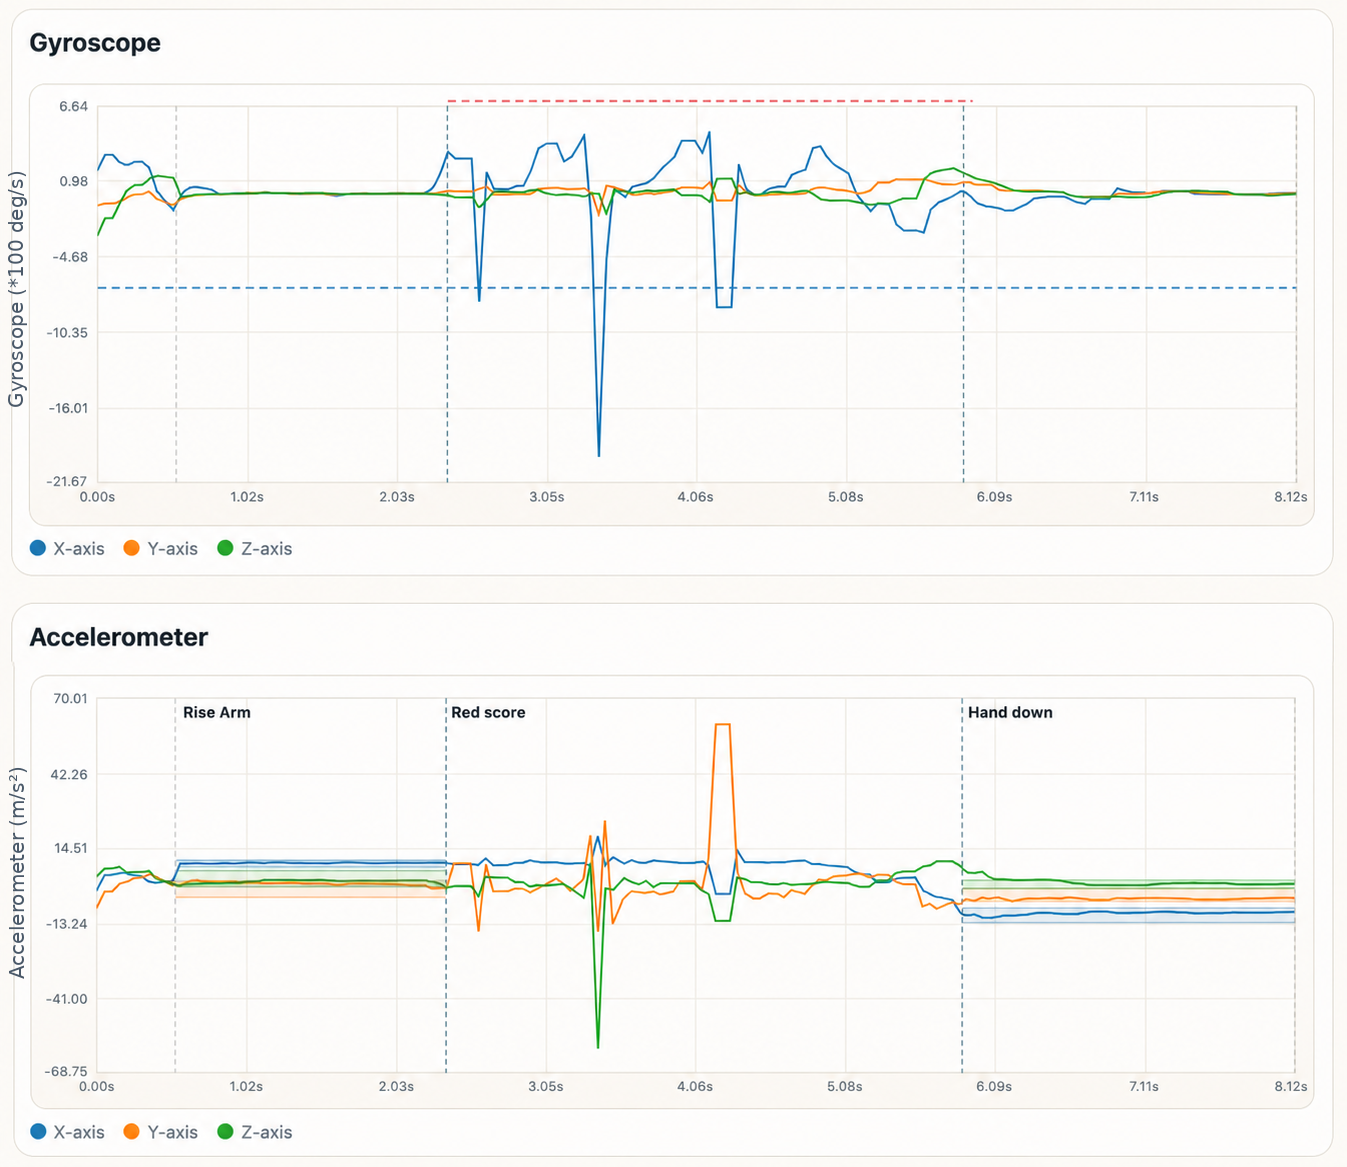
\includegraphics[width=0.95\textwidth]{img/gesture-flow/flow-gesto-bodovanie.png}
  \caption{Priebeh gyroskopických a~akcelerometrických dát počas celého gesta BODOVANIE pre červeného zápasníka.}
  \label{fig:bodovanie-priebeh}
\end{figure}

Na obrázku~\ref{fig:bodovanie-priebeh} sú zvislými prerušovanými čiarami vyznačené tri kľúčové
momenty zodpovedajúce trom fázam gesta. V~prvej fáze (\uv{Rise Arm}) sa hodnoty akcelerometra
ustália v~rozsahoch zodpovedajúcich zdvihnutej polohe ruky, čím sa aplikácia prepne do režimu
bodovania pre červeného zápasníka. V~druhej fáze (\uv{Red score}) je v~hornej časti grafu
viditeľný výrazný záporný špičkový výkyv na osi $g_x$ (modrá), ktorý prekračuje prahovú hodnotu
$\flckBlueThreshold\,\text{DPS}$ a~spôsobí pridelenie bodu. V~tretej fáze (\uv{Hand Down}) sa
hodnoty akcelerometra ustália v~rozsahoch zodpovedajúcich neutrálnej polohe ruky, čo signalizuje
ukončenie procesu bodovania.

Z~grafu je tiež zrejmé, že v~strednej fáze rozhodca
vykonal tri po sebe nasledujúce flicky a~aplikácia
pridala tri body červenému zápasníkovi.

Obdobne by vyzeral priebeh gesta \uv{Bodovanie} pre modrého zápasníka, s~tým rozdielom, že aktivácia by prebehla gestom \uv{Hand Back}
a~flicky by pridávali body modrému zápasníkovi.

\subsection{Gesto PASIVITA}

Gesto \uv{Pasivita} slúži na signalizáciu pasívneho
správania jedného zo zápasníkov bodovému rozhodcovi.
Pre toto gesto sme navrhli dve alternatívy -- pre
červeného a~modrého zápasníka.

Pôvodný návrh počítal s~automatickým 30-sekundovým
odpočtom po detekcii gesta -- ak by žiaden zo zápasníkov
počas tejto doby neskóroval, aplikácia by automaticky
pridelila 1~bod súperovi pasívneho zápasníka. Tento
priebeh je znázornený vo vývojovom diagrame na
obrázku~\ref{fig:pasivita-flowchart}.

\begin{figure}[H]
  \centering
  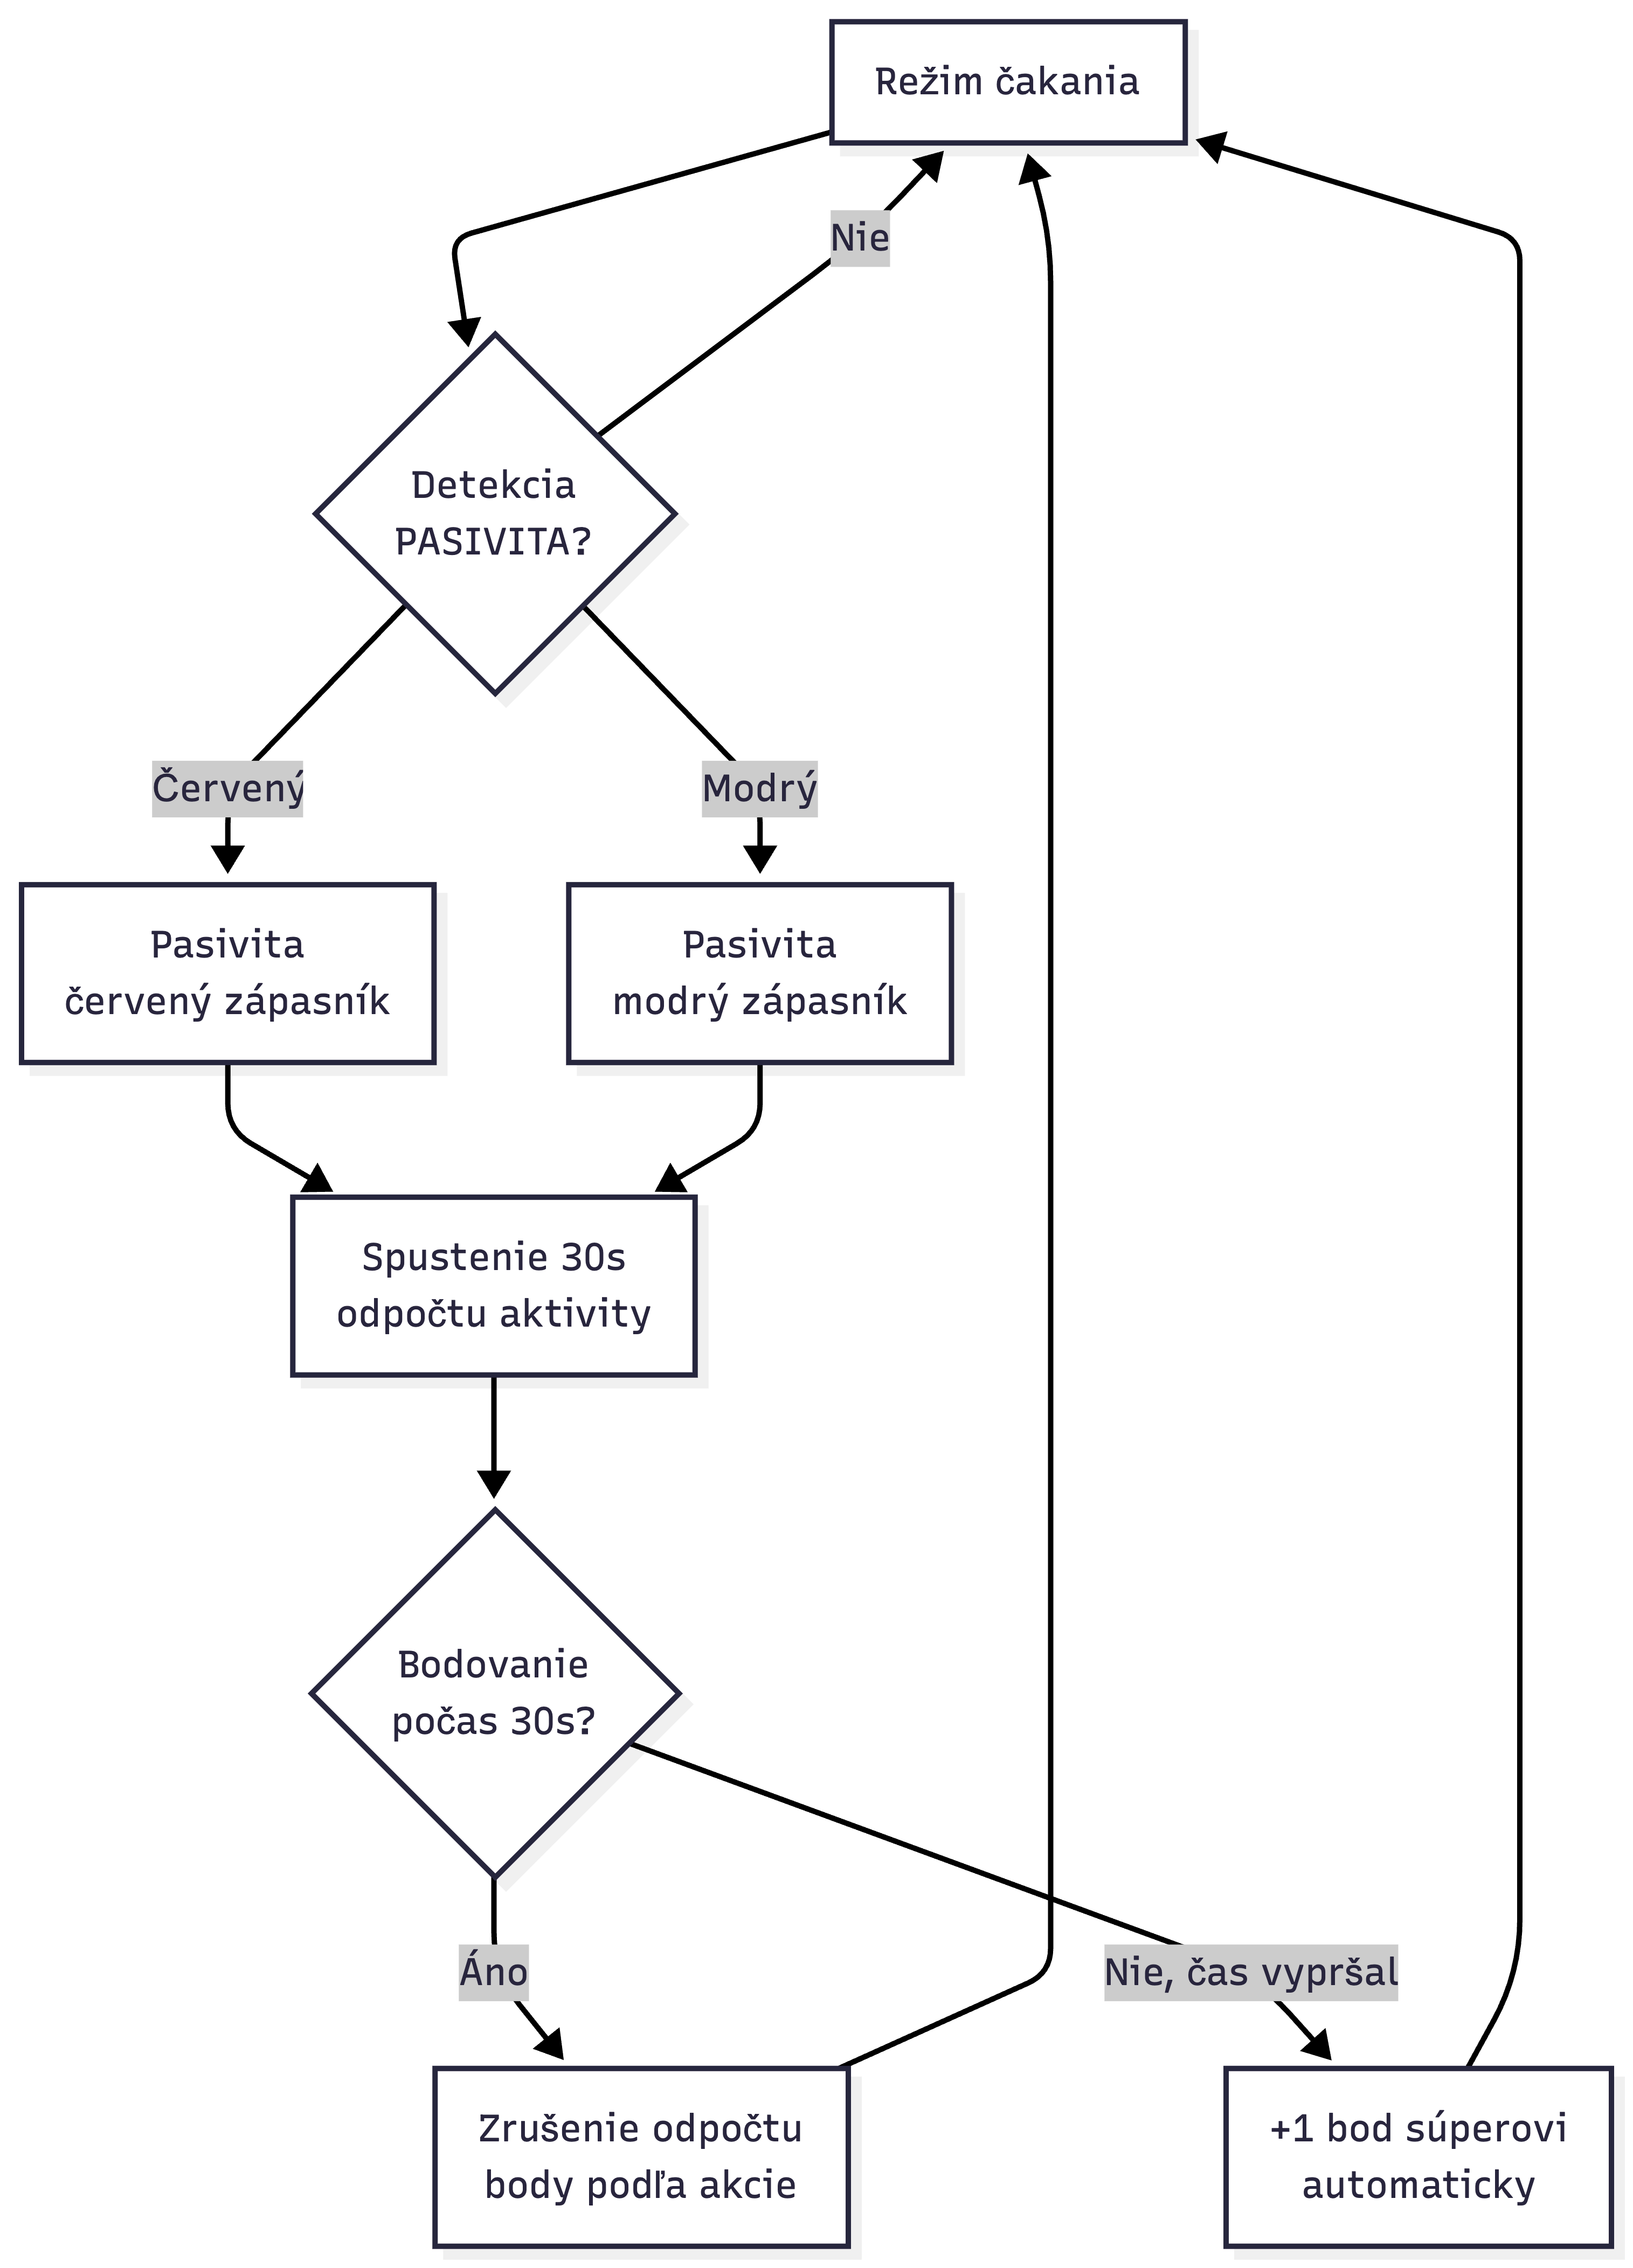
\includegraphics[width=0.6\textwidth]{img/diagrams/flowchart-gesto-pasivita.png}
  \caption{Pôvodne navrhovaný vývojový diagram gesta PASIVITA s~automatickým odpočtom}
  \label{fig:pasivita-flowchart}
\end{figure}

Po zvážení reálnych podmienok zápasu sme tento
mechanizmus implementovali iba v~debug móde aplikácie.
V~produkčnom móde gesto \uv{Pasivita} pasivitu len
zaznamená ako udalosť. Detailné dôvody tohto rozhodnutia
sú uvedené v~kapitole~\ref{chapter:implementacia}
v~rámci popisu produkčného módu
(podsekcia~\ref{app:prod-final}).

\subsubsection{PASIVITA -- červený}

Rozhodca vystrčí ľavú ruku (s~hodinkami) vodorovne
do strany v~90-stupňovom uhle od tela, pričom dlaň
smeruje nadol k~zemi.

\begin{figure}[H]
  \centering
  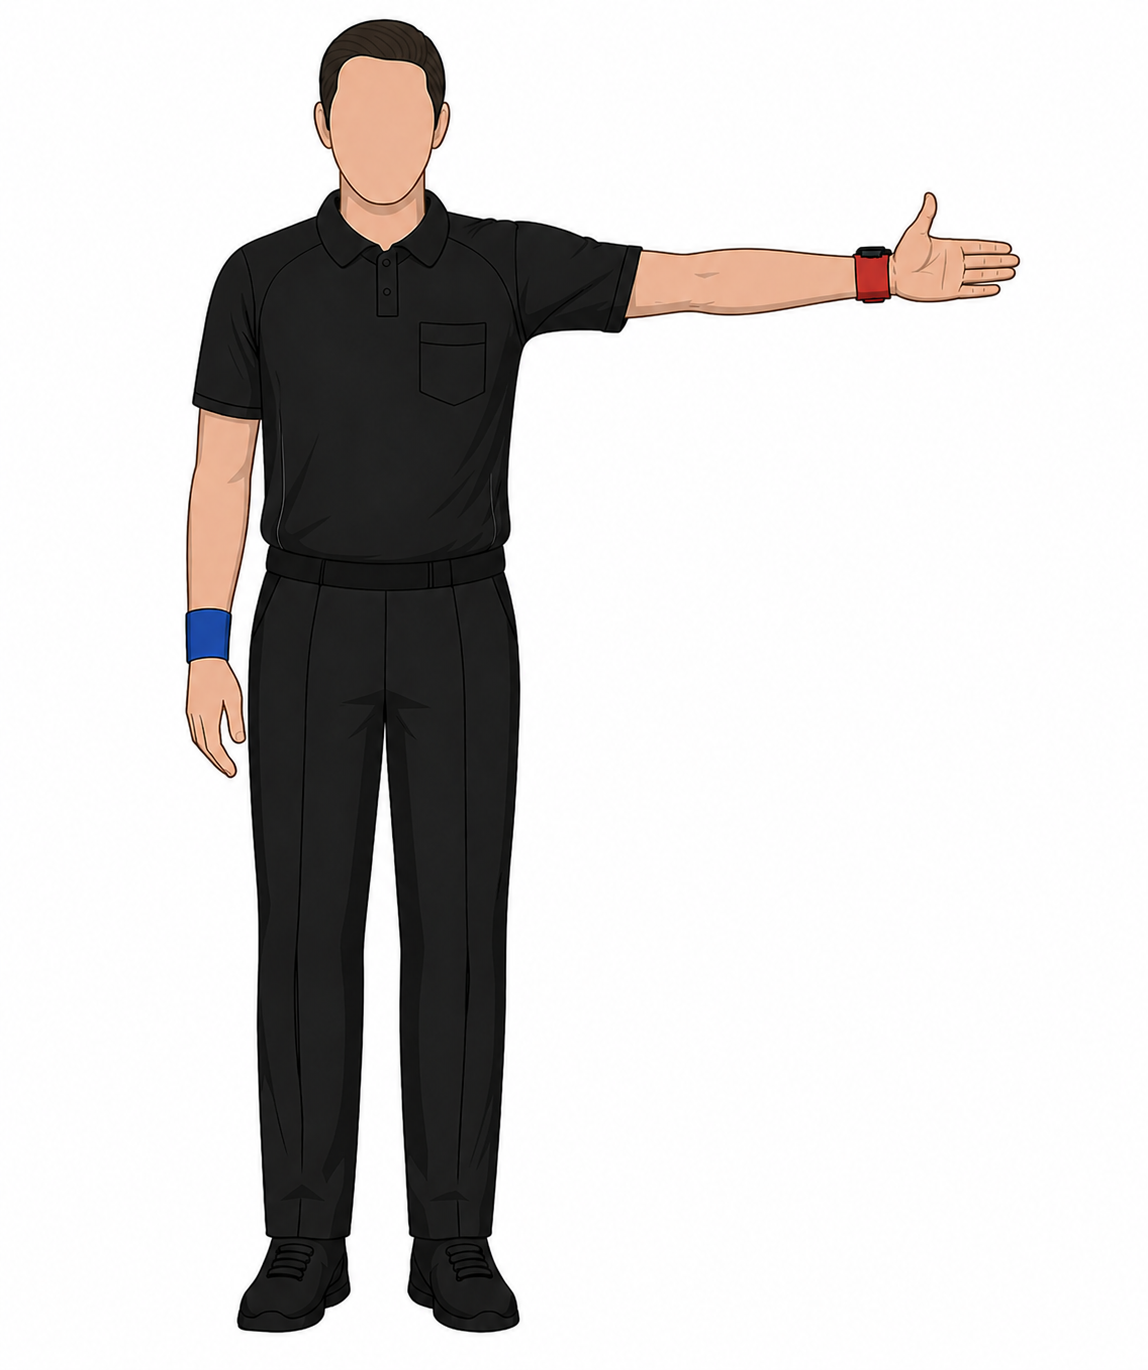
\includegraphics[width=0.4\textwidth]{img/gesture-img/obrazok-gesto-pasivity-cerveny.png}
  \caption{Poloha ruky pri geste
    \uv{PASIVITA -- červený}}
  \label{fig:gesto-pasivita-cerveny}
\end{figure}

\begin{figure}[H]
  \centering
  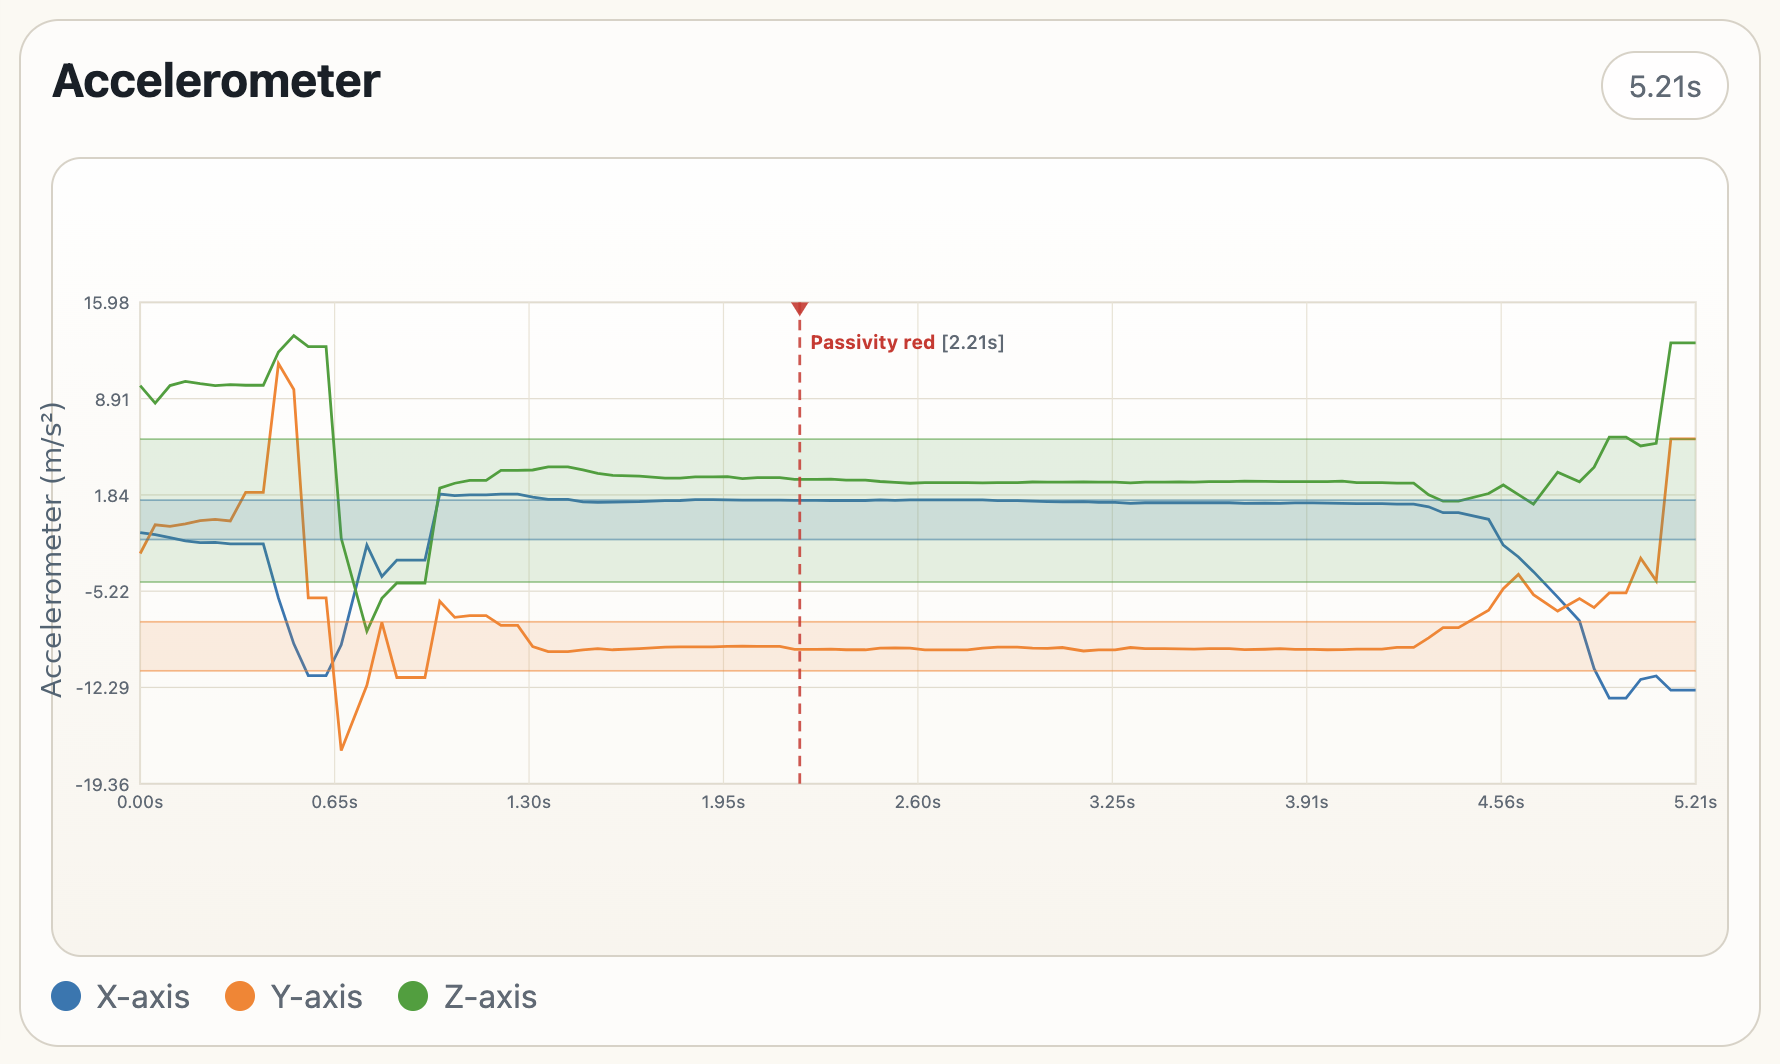
\includegraphics[width=0.9\textwidth]{img/gesture-flow/flow-gesto-pasivita-cerveny.png}
  \caption{Akcelerometrické dáta gesta \uv{PASIVITA -- červený}}
  \label{fig:subgesture-pasivita-cerveny}
\end{figure}

Na obrázku~\ref{fig:subgesture-pasivita-cerveny}
je zobrazený priebeh akcelerometrických dát počas
vykonania aktivačného gesta \uv{PASIVITA -- červený}.
Farebné pásma znázorňujú
očakávaný interval hodnôt pre jednotlivé osi
v~cieľovej polohe.

\noindent
\textbf{Interval hodnôt:}

\begin{itemize}
  \item \colorbox{xaxis!20}{$\passivityRedAxMin \leq a_x \leq \passivityRedAxMax \;\text{m/s}^2$}
  \item \colorbox{yaxis!20}{$\passivityRedAyMin \leq a_y \leq \passivityRedAyMax \;\text{m/s}^2$}
  \item \colorbox{zaxis!20}{$\passivityRedAzMin \leq a_z \leq \passivityRedAzMax \;\text{m/s}^2$}
\end{itemize}

\subsubsection{PASIVITA -- modrý}

Rozhodca vystrčí ľavú ruku (s~hodinkami) vodorovne
dopredu pred telo, pričom dlaň smeruje nahor
k~stropu.

\begin{figure}[H]
  \centering
  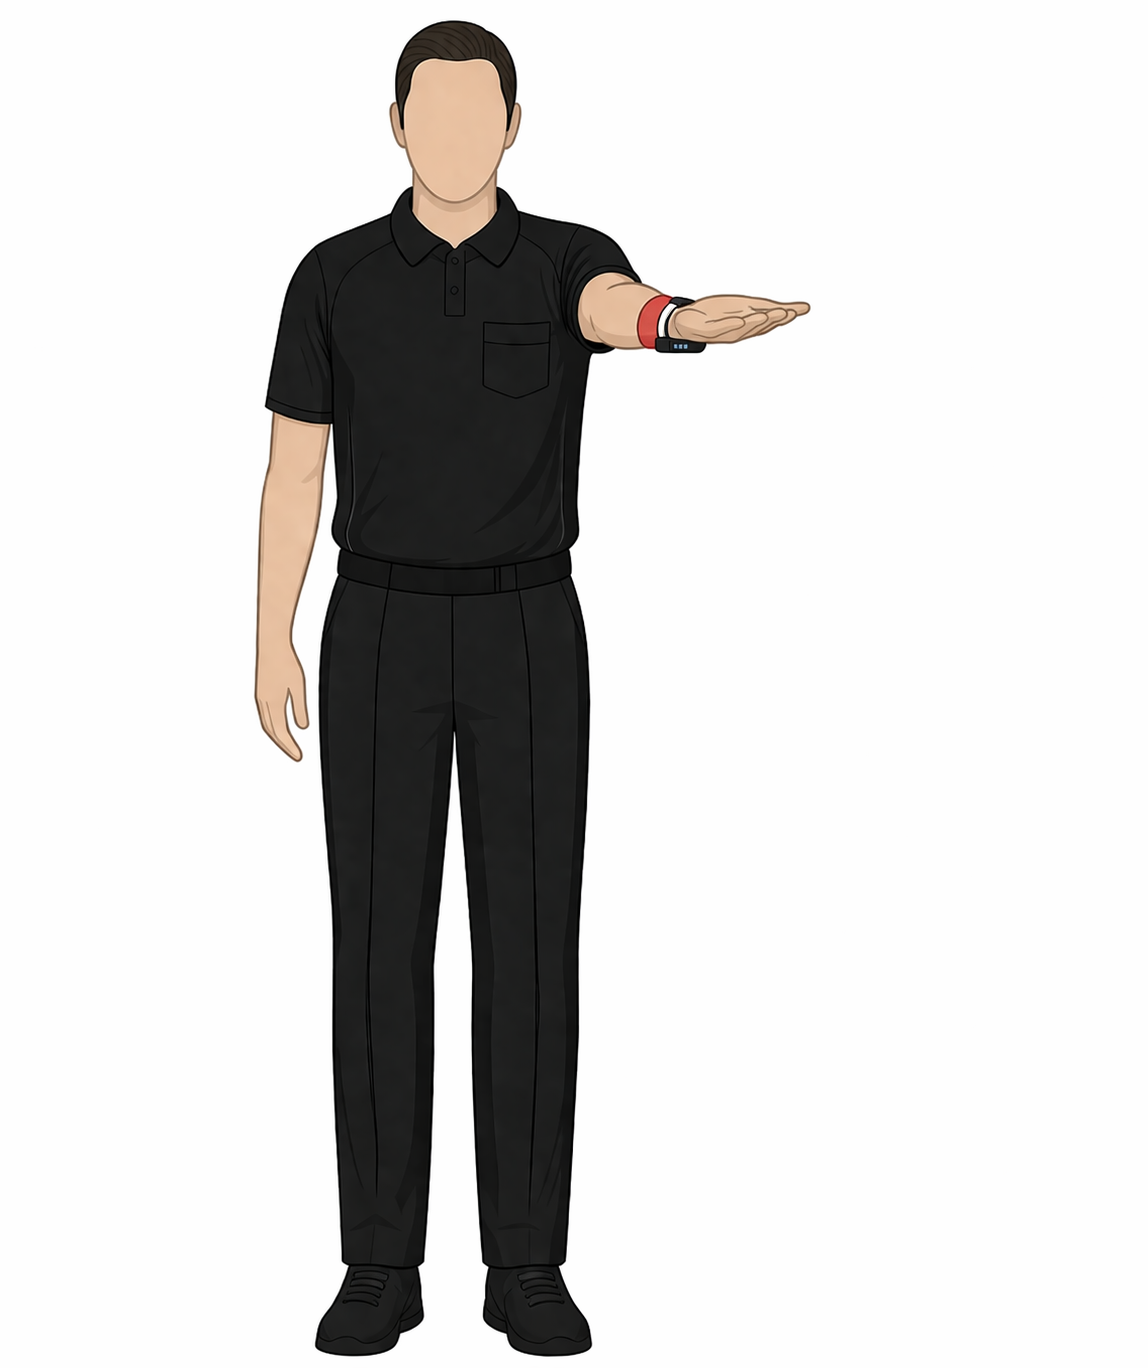
\includegraphics[width=0.4\textwidth]{img/gesture-img/obrazok-gesto-pasivity-modry.png}
  \caption{Poloha ruky s hodinkami pri geste
    \uv{PASIVITA -- modrý} -- poloha ruky s modrou manžetou nezodpovedá skutočnej polohe ruky rozhodcu počas zápasu.}
  \label{fig:gesto-pasivita-modry}
\end{figure}

\begin{figure}[H]
  \centering
  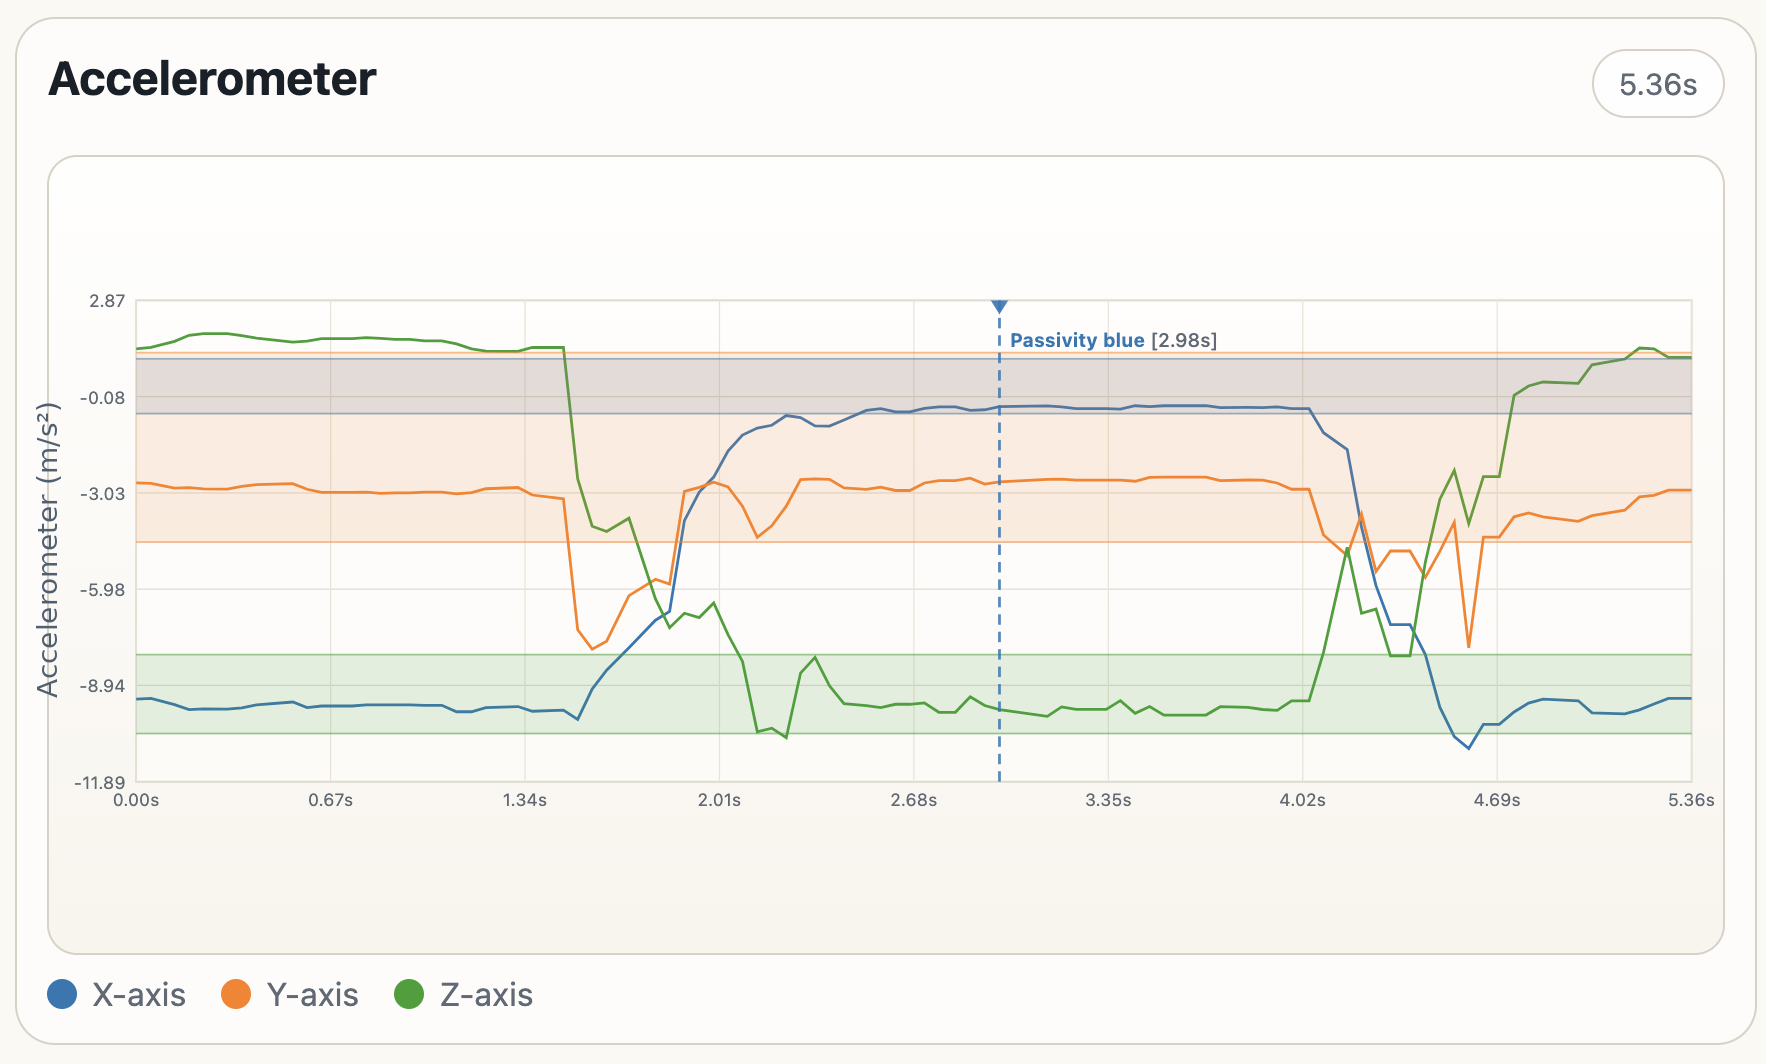
\includegraphics[width=0.9\textwidth]{img/gesture-flow/flow-gesto-pasivita-modry.png}
  \caption{Akcelerometrické dáta gesta \uv{PASIVITA -- modrý}}
  \label{fig:subgesture-pasivita-modry}
\end{figure}

Na obrázku~\ref{fig:subgesture-pasivita-modry}
je zobrazený priebeh akcelerometrických dát počas
vykonania gesta \uv{PASIVITA -- modrý}. Farebné pásma znázorňujú
očakávaný interval hodnôt pre jednotlivé osi
v~cieľovej polohe.

\noindent
\textbf{Interval hodnôt:}

\begin{itemize}
  \item \colorbox{xaxis!20}{$\passivityBlueAxMin \leq a_x \leq \passivityBlueAxMax \;\text{m/s}^2$}
  \item \colorbox{yaxis!20}{$\passivityBlueAyMin \leq a_y \leq \passivityBlueAyMax \;\text{m/s}^2$}
  \item \colorbox{zaxis!20}{$\passivityBlueAzMin \leq a_z \leq \passivityBlueAzMax \;\text{m/s}^2$}
\end{itemize}

\subsection{Gesto NAPOMENUTIE}

Gesto \uv{Napomenutie} slúži na signalizáciu
priestupku zápasníka (podrobne popísané
v~kapitole~\ref{chapter:zapasenie}). Po detekcii aplikácia automaticky prepne do režimu
bodovania, kde sú všetky body pripočítavané výhradne
súperovi napomenutého zápasníka. Rozhodca následne
počtom vykonaní gesta \uv{Flick} určí počet udelených
bodov. Po ukončení bodovania je potrebné vykonať gesto
\uv{Hand Down}, ktoré vráti aplikáciu späť do režimu
čakania.

\begin{figure}[H]
  \centering
  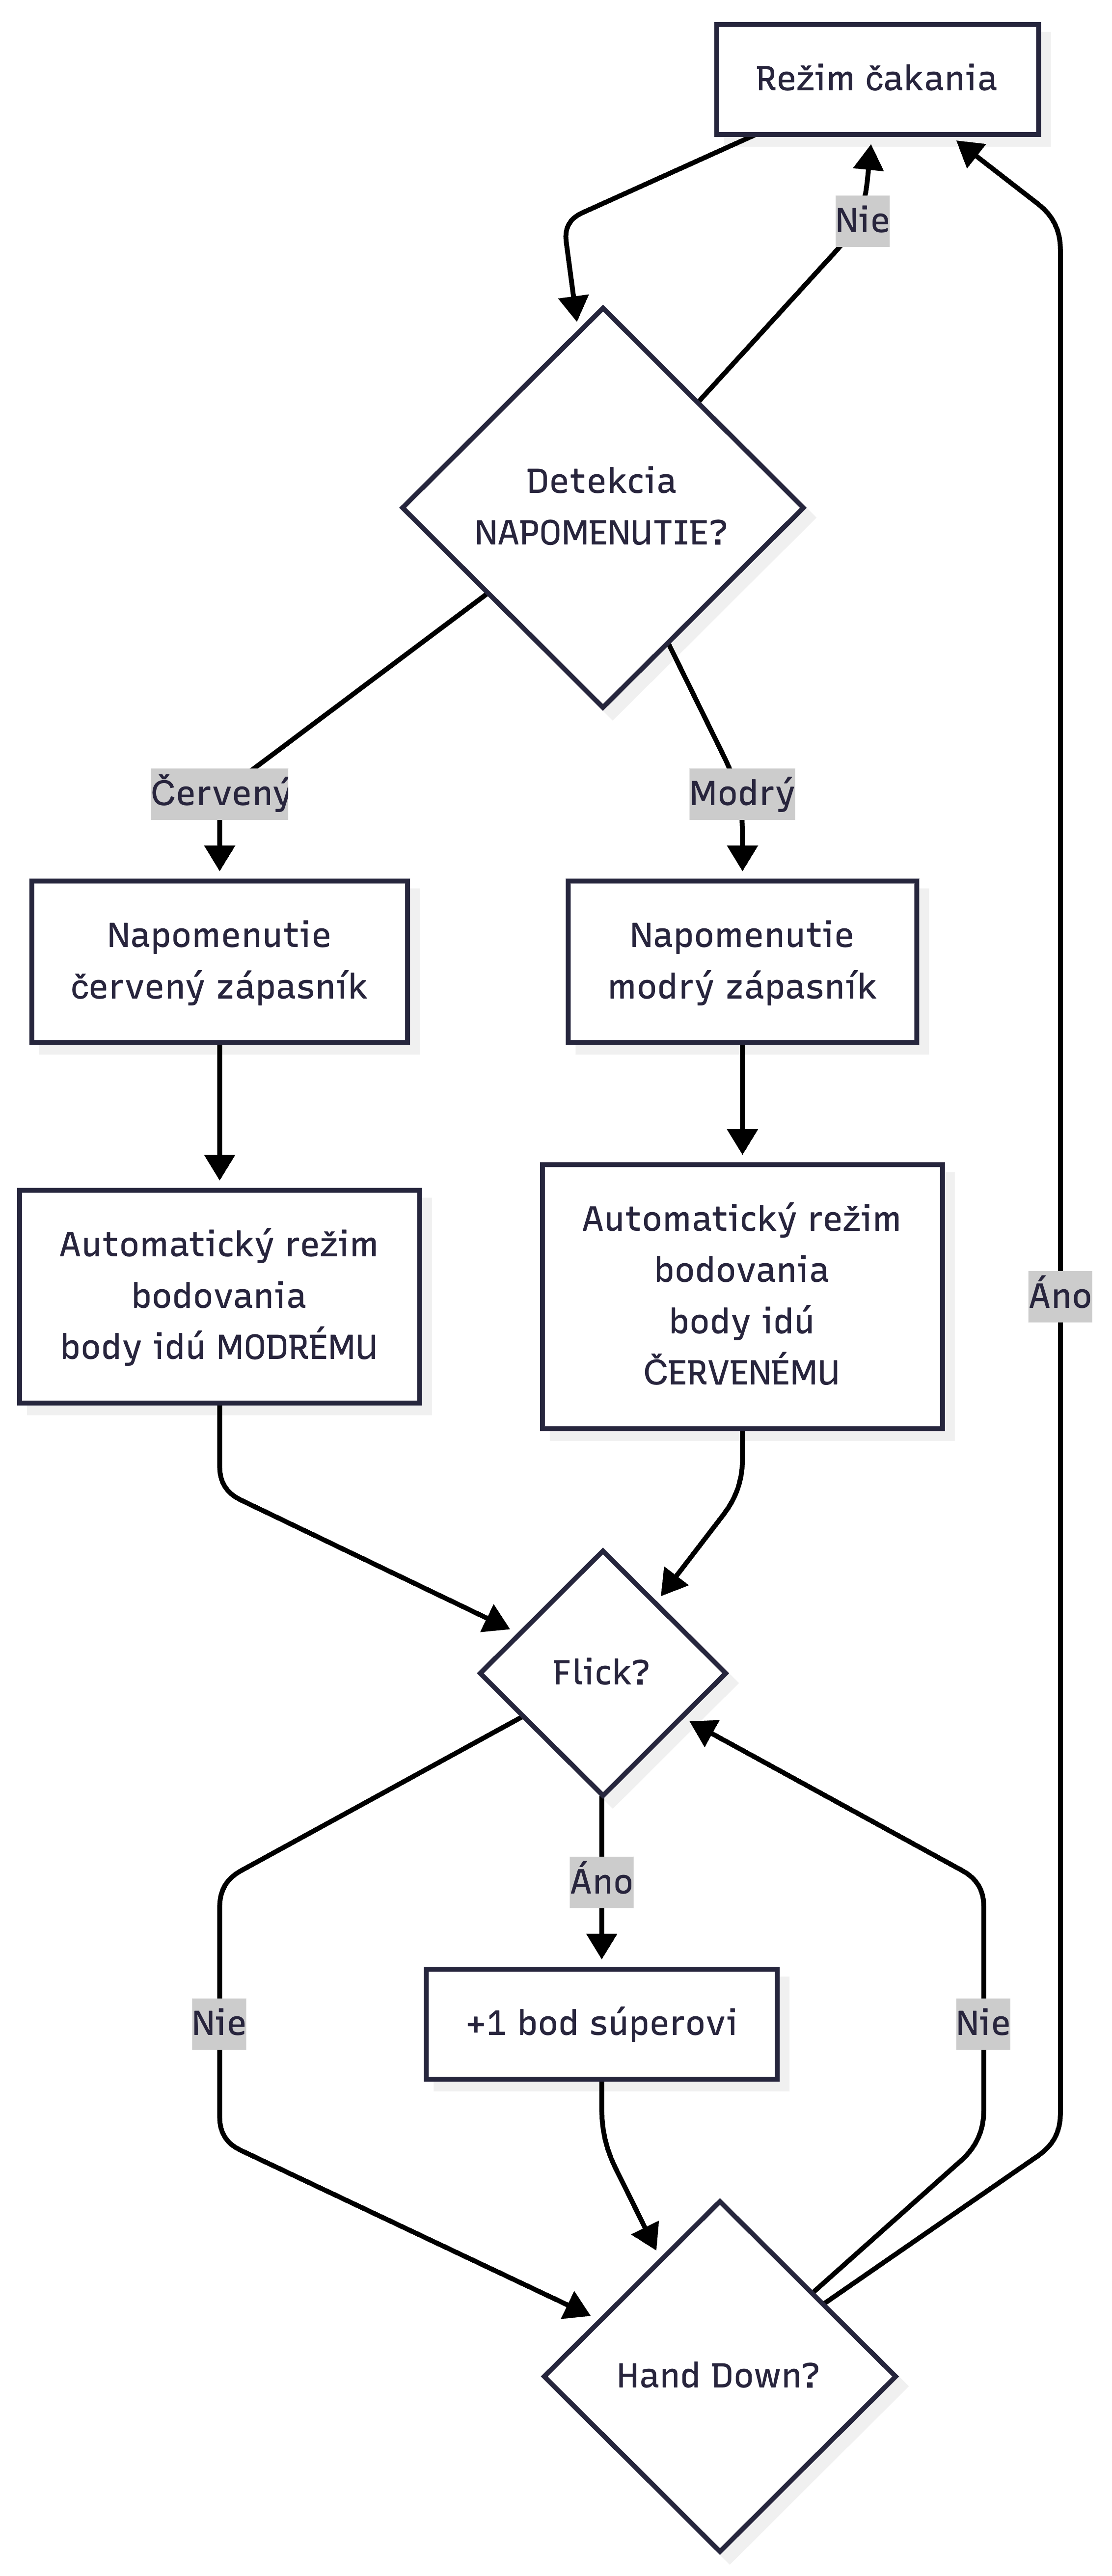
\includegraphics[width=0.6\textwidth]{img/diagrams/flowchart-gesto-napomenutie.png}
  \caption{Vývojový diagram gesta NAPOMENUTIE}
  \label{fig:napomenutie-flowchart}
\end{figure}

\subsubsection{NAPOMENUTIE -- červený}

Rozhodca vystrčí ľavú ruku (s~hodinkami) šikmo
dopredu a~nadol pod uhlom približne 45°, pričom dlaň
smeruje nadol. Gestom ukazuje na previnilého
červeného zápasníka. Po detekcii sa aplikácia
automaticky prepne do režimu bodovania, kde všetky
body idú modrému zápasníkovi.

\begin{figure}[H]
  \centering
  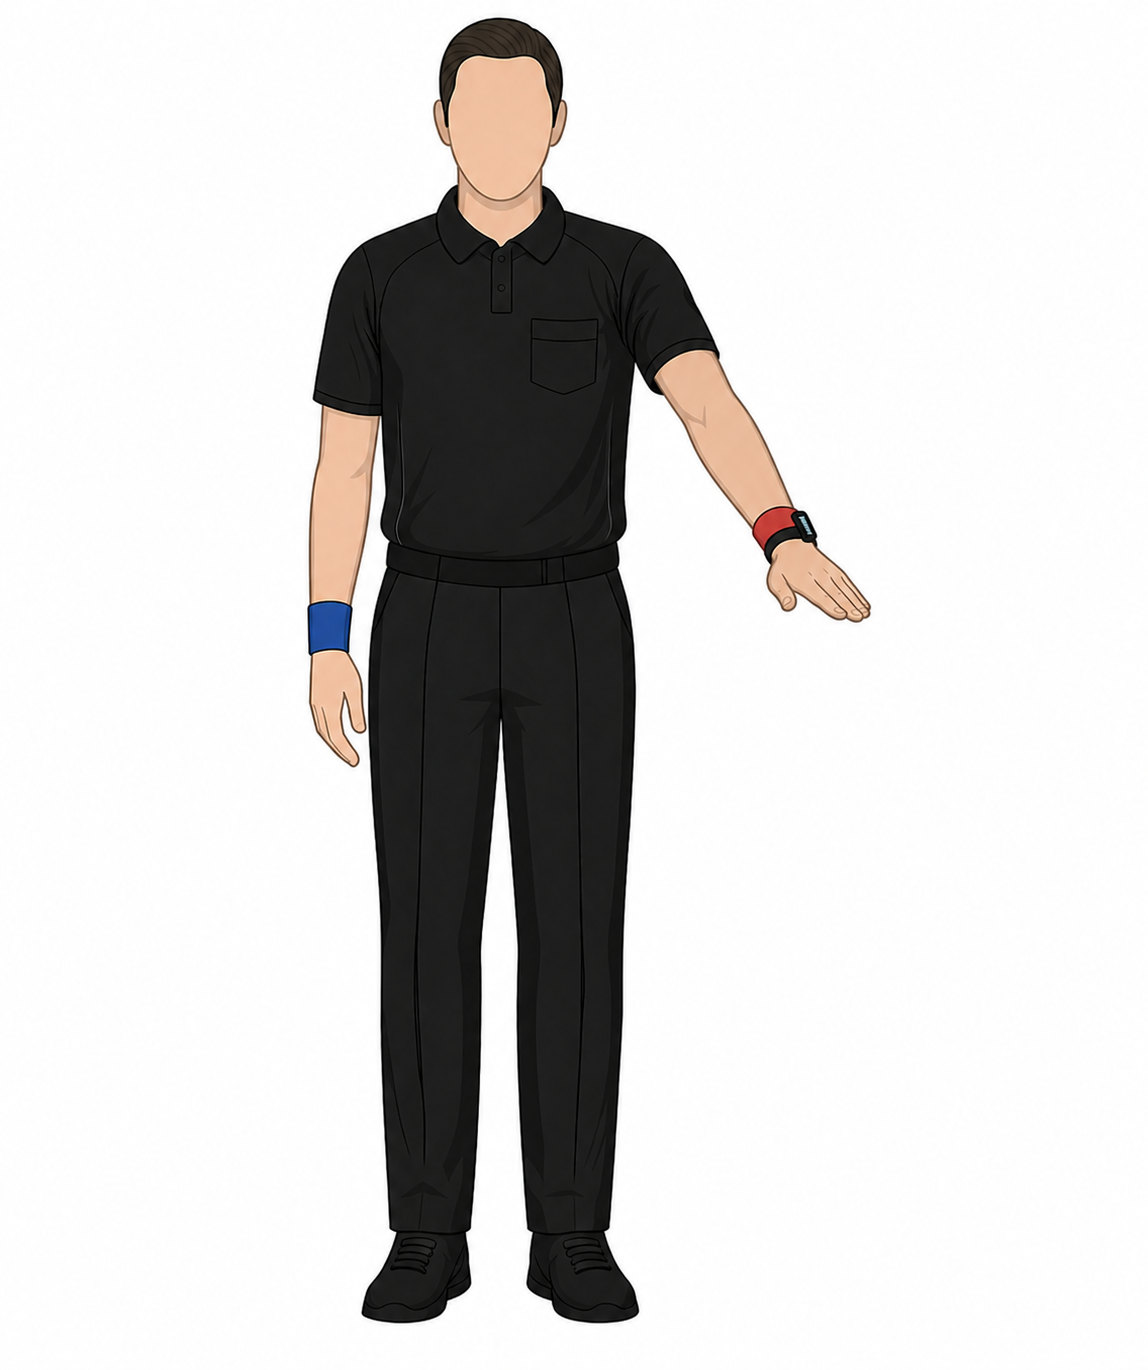
\includegraphics[width=0.4\textwidth]{img/gesture-img/obrazok-gesto-napomenutie-cerveny.png}
  \caption{Poloha ruky pri geste
    \uv{NAPOMENUTIE -- červený}}
  \label{fig:gesto-napomenutie-cerveny}
\end{figure}
\begin{figure}[H]
  \centering
  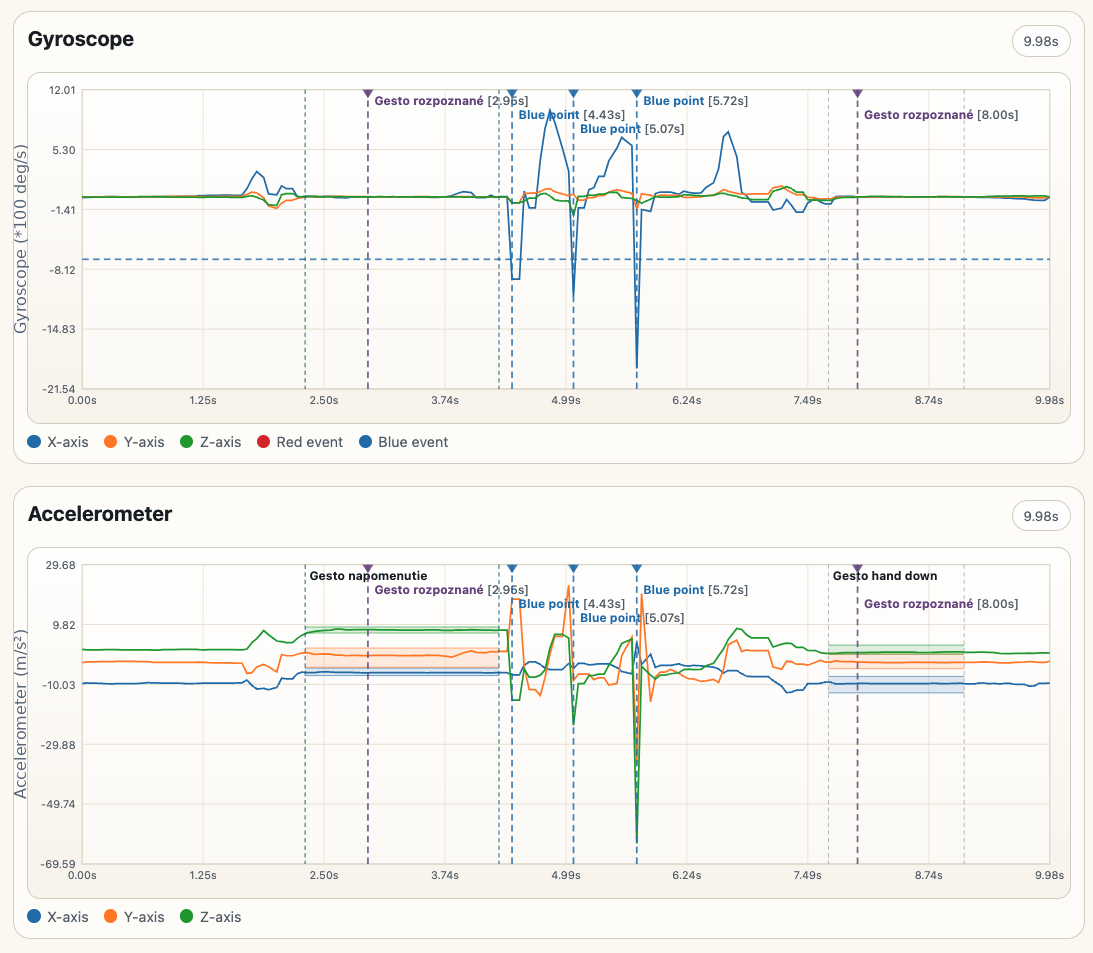
\includegraphics[width=0.9\textwidth]{img/gesture-flow/flow-gesto-napomenutie-cerveny.png}
  \caption{Priebeh gesta \uv{NAPOMENUTIE -- červený} s~následným bodovaním}
  \label{fig:subgesture-napomenutie-cerveny}
\end{figure}

Na obrázku~\ref{fig:subgesture-napomenutie-cerveny} je zobrazený priebeh
gyroskopických a~akcelerometrických dát počas vykonania aktivačného gesta
\uv{NAPOMENUTIE -- červený} a~následnej sekvencie bodovania. V~prvej fáze
(\uv{Gesto napomenutie}) sa aplikácia
prepne do režimu napomenutia červeného zápasníka. V~druhej fáze rozhodca
vykonal tri po sebe nasledujúce gestá \uv{Flick}, ktoré sú v~hornej časti grafu
viditeľné ako výrazné záporné špičkové výkyvy na osi $g_x$ (modrá)
prekračujúce prahovú hodnotu $\flckBlueThreshold\,\text{DPS}$. Každý
z~týchto výkyvov pridelil jeden bod modrému zápasníkovi, keďže bodovanie
je v~režime napomenutia obmedzené len na súpera napomenutého
zápasníka. V~tretej fáze (\uv{Hand Down}) sa hodnoty
akcelerometra ustália v~rozsahoch zodpovedajúcich polohe gesta \uv{Hand Down},
čo signalizuje ukončenie procesu napomenutia červeného zápasníka.

Pre os $a_y$ (oranžová) sme zvolili väčší rozsah, pretože ruka rozhodcu
nemusí smerovať presne dole -- pri reálnom použití môže dochádzať
k~jemnému odklonu od ideálnej polohy. Farebné pásma na grafe akcelerometra
znázorňujú očakávaný interval hodnôt pre jednotlivé osi v~cieľovej polohe
aktivačného gesta \uv{NAPOMENUTIE -- červený} a~v~neutrálnej polohe gesta
\uv{Hand Down}.

\noindent
\textbf{Interval hodnôt:}

\begin{itemize}
  \item \colorbox{xaxis!20}{$\warnRedAxMin \leq a_x \leq \warnRedAxMax \;\text{m/s}^2$}
  \item \colorbox{yaxis!20}{$\warnRedAyMin \leq a_y \leq \warnRedAyMax \;\text{m/s}^2$}
  \item \colorbox{zaxis!20}{$\warnRedAzMin \leq a_z \leq \warnRedAzMax \;\text{m/s}^2$}
\end{itemize}

\subsubsection{NAPOMENUTIE -- modrý}

Pri napomenutí modrého zápasníka rozhodca pokrčí ľavú ruku (s~hodinkami)
v~lakti pred bruchom, pričom predlaktie je vodorovne a~otvorená dlaň
smeruje šikmo nahor. Pravou rukou (s~modrou manžetou) ukazuje na previnilého
modrého zápasníka. Po detekcii sa aplikácia automaticky prepne do režimu
bodovania, kde všetky body idú červenému zápasníkovi.

\begin{figure}[H]
  \centering
  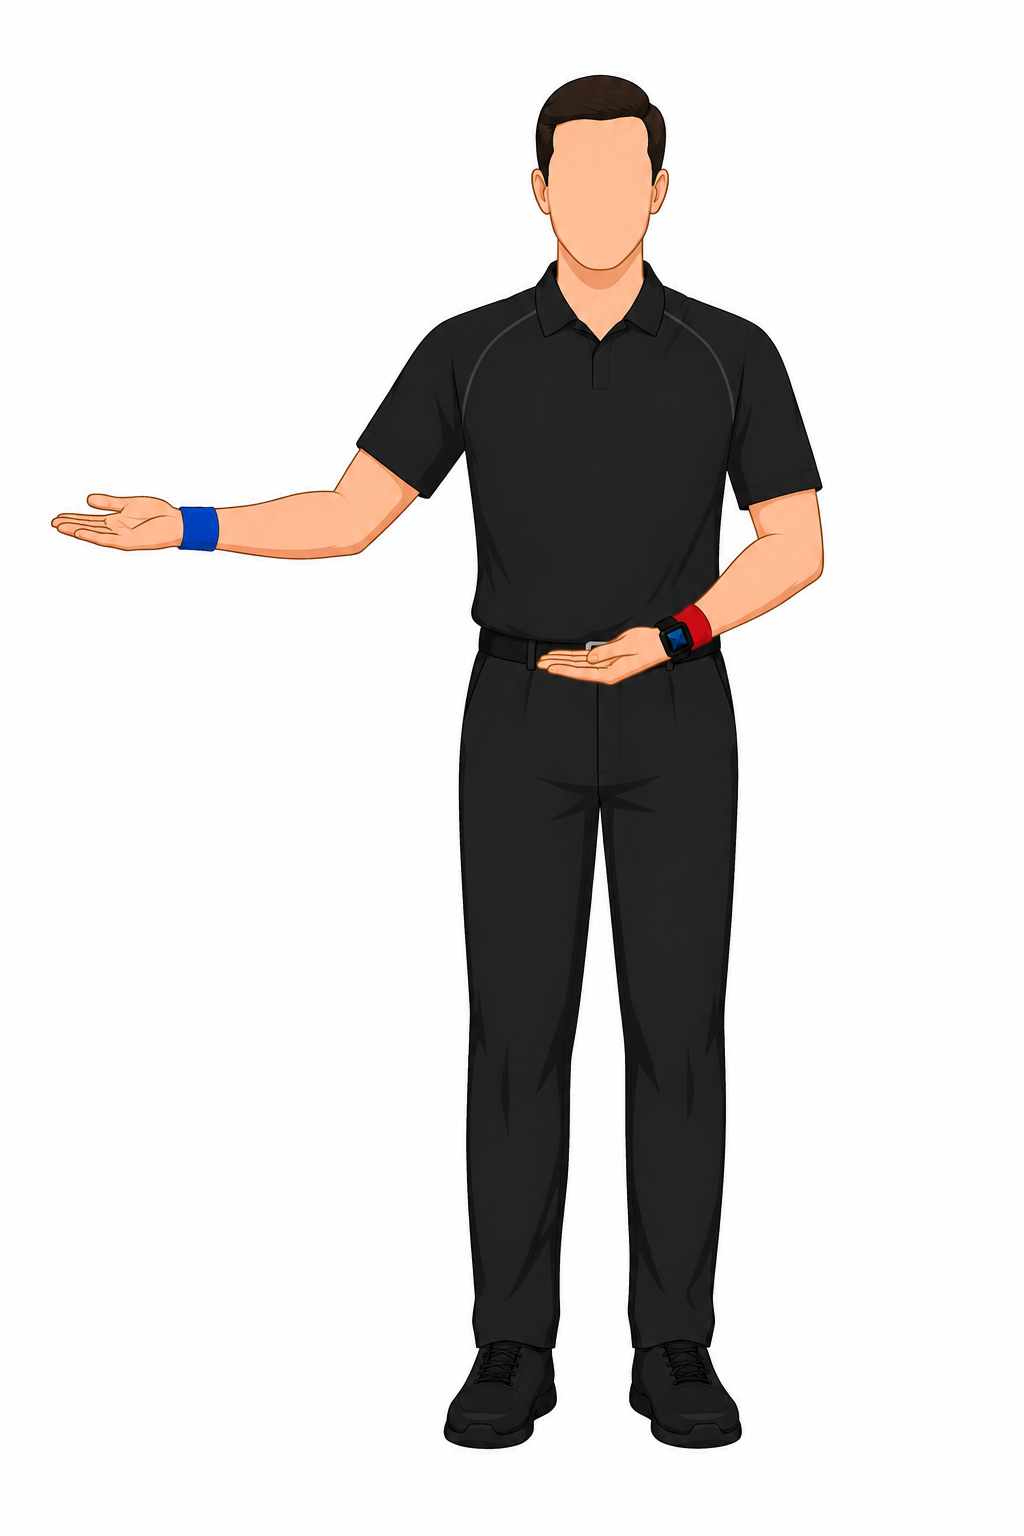
\includegraphics[width=0.5\textwidth]{img/gesture-img/obrazok-gesto-napomenutie-modry1.png}
  \caption{Poloha ruky pri geste \uv{NAPOMENUTIE -- modrý}}
  \label{fig:gesto-napomenutie-modry}
\end{figure}

\begin{figure}[H]
  \centering
  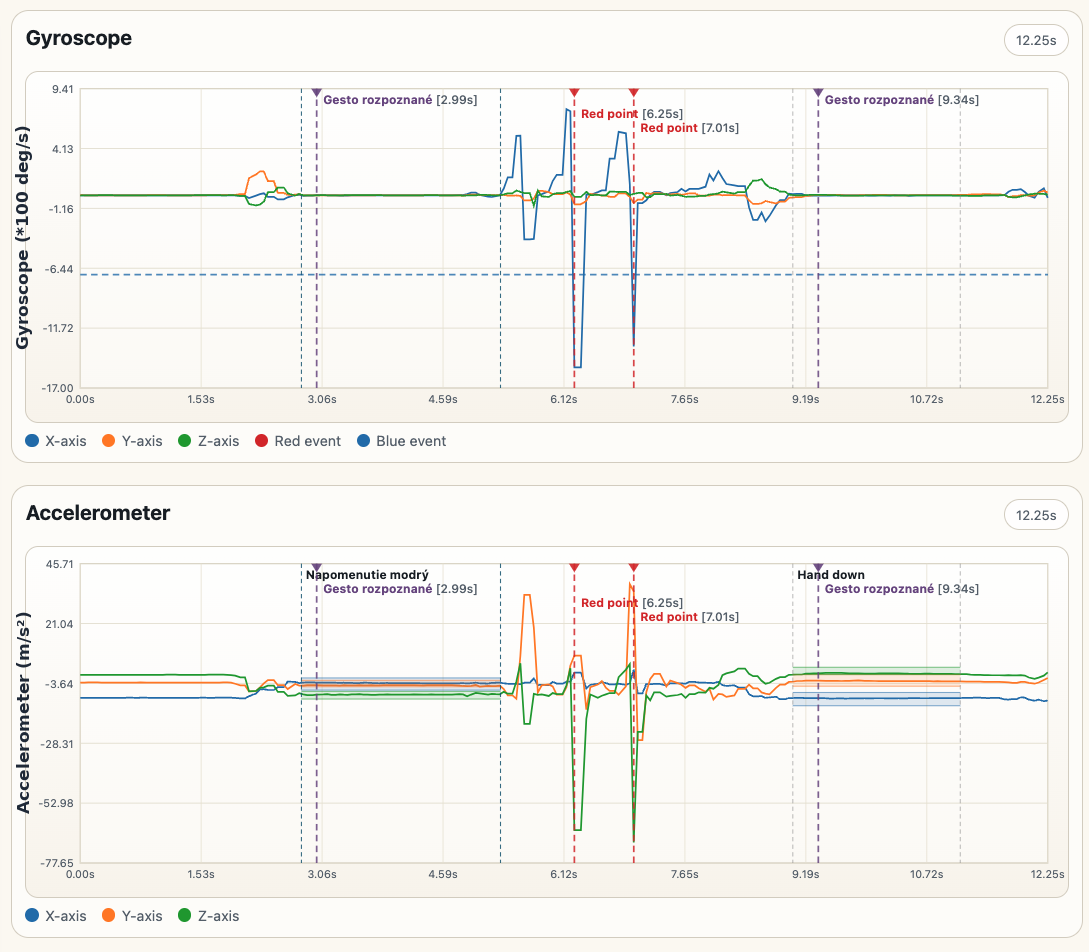
\includegraphics[width=0.9\textwidth]{img/gesture-flow/flow-gesto-napomenutie-modry.png}
  \caption{Priebeh gesta \uv{NAPOMENUTIE -- modrý} s~následným bodovaním}
  \label{fig:subgesture-napomenutie-modry}
\end{figure}

Na obrázku~\ref{fig:subgesture-napomenutie-modry} je zobrazený priebeh
gyroskopických a~akcelerometrických dát počas vykonania aktivačného gesta
\uv{NAPOMENUTIE -- modrý} a~následnej sekvencie bodovania. V~prvej fáze (\uv{Gesto napomenutie}) sa aplikácia
prepne do režimu napomenutia modrého zápasníka.
V~druhej fáze rozhodca vykonal dve po sebe nasledujúce gestá \uv{Flick}.
Každé z~nich pridelilo jeden bod červenému zápasníkovi.

V~tretej fáze (\uv{Hand Down}) sa hodnoty
akcelerometra ustália v~rozsahoch zodpovedajúcich polohe gesta \uv{Hand Down},
čo signalizuje ukončenie procesu napomenutia modrého zápasníka.

\noindent
\textbf{Interval hodnôt:}

\begin{itemize}
  \item \colorbox{xaxis!20}{$\warnBlueAxMin \leq a_x \leq \warnBlueAxMax \;\text{m/s}^2$}
  \item \colorbox{yaxis!20}{$\warnBlueAyMin \leq a_y \leq \warnBlueAyMax \;\text{m/s}^2$}
  \item \colorbox{zaxis!20}{$\warnBlueAzMin \leq a_z \leq \warnBlueAzMax \;\text{m/s}^2$}
\end{itemize}

Hoci je poloha ruky pri tomto geste podobná
gestu \uv{PASIVITA -- modrý} (obe gestá majú dlaň
otočenú nahor a~ruku vodorovne pred telom),
kľúčový rozdiel je v~ohybe v~lakti. Pri \uv{PASIVITA
-- modrý} je ruka úplne vystretá pred telom,
pri \uv{NAPOMENUTIE -- modrý} je pokrčená v~lakti
s~predlaktím nad bruchom.

\subsection{Gesto TOUCHE}

Gesto \uv{TOUCHE} slúži na signalizáciu lopatkového
víťazstva, ktoré v~reálnom zápase okamžite ukončuje
zápas (podrobne popísané v~kapitole~\ref{chapter:zapasenie}).
V~našej aplikácii sa však TOUCHE zaznamenáva iba
ako informačný záznam, keďže o~jeho platnosti
rozhoduje predseda žinenky mimo systému hodiniek
(viď podsekciu~\ref{subsec:analyza-informaticka}).
Keďže je vždy jednoznačné, ktorý zápasník je na
lopatkách, pre toto gesto stačí jedna alternatíva
bez rozlíšenia červeného a~modrého zápasníka.

Rozhodca preloží ľavú ruku (s~hodinkami) cez hruď
a~položí dlaň na pravé rameno.
Na obrázku~\ref{fig:gesto-touche} je znázornená
poloha ruky pri tomto geste.

\begin{figure}[H]
  \centering
  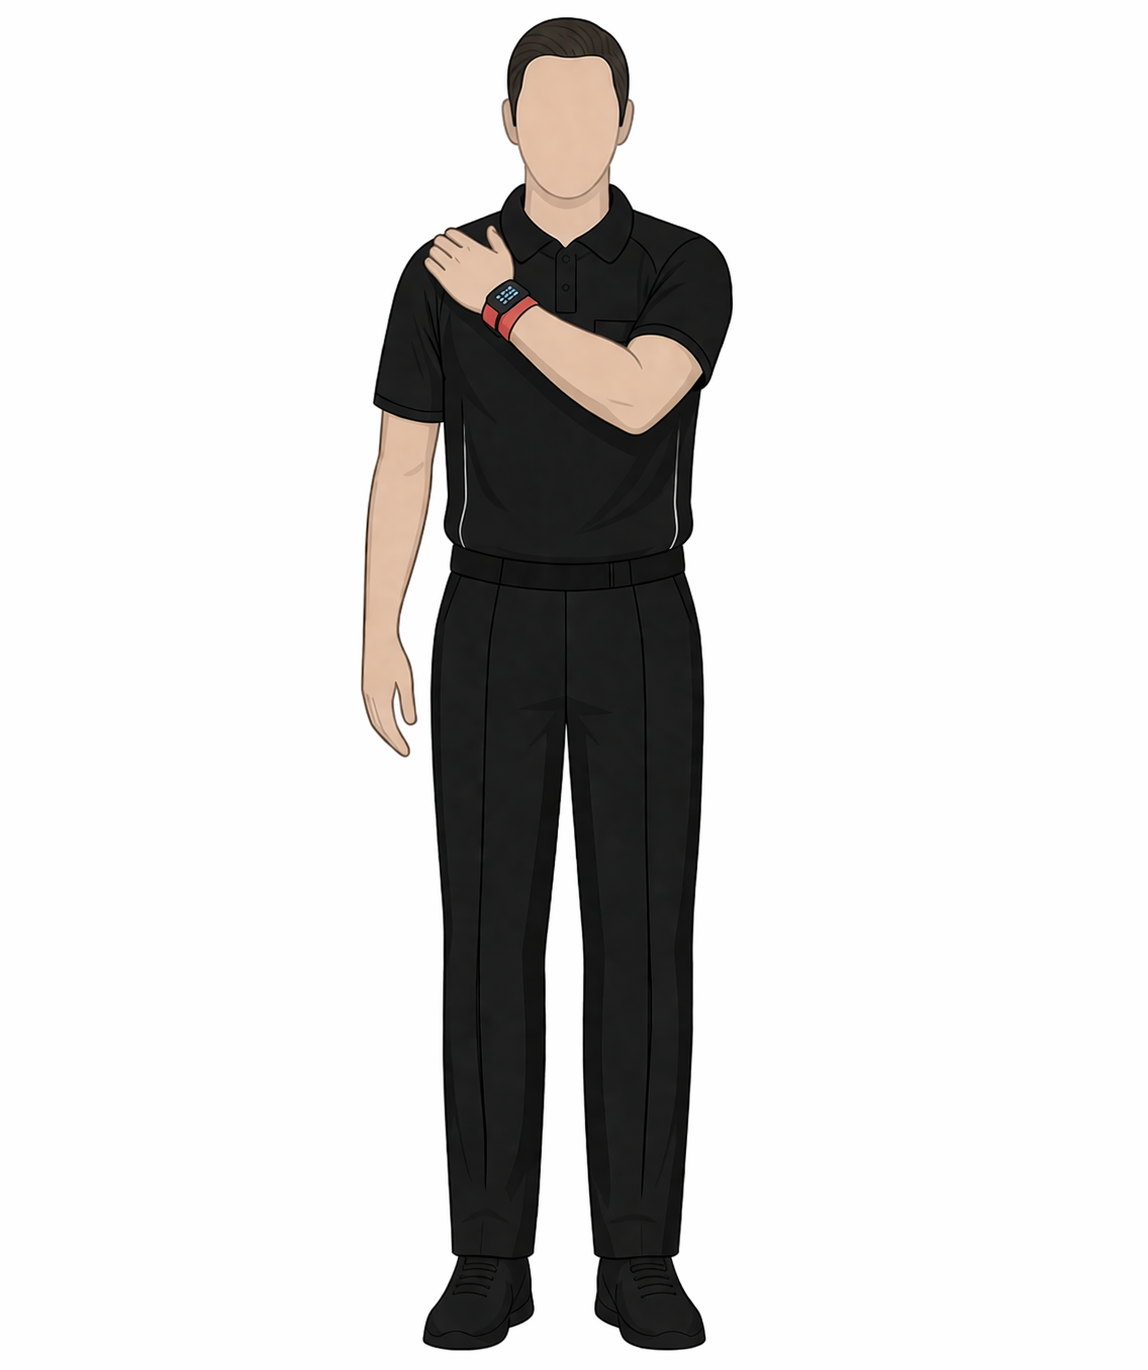
\includegraphics[width=0.4\textwidth]{img/gesture-img/obrazok-gesto-touche.png}
  \caption{Poloha ruky pri geste \uv{TOUCHE}}
  \label{fig:gesto-touche}
\end{figure}

\begin{figure}[H]
  \centering
  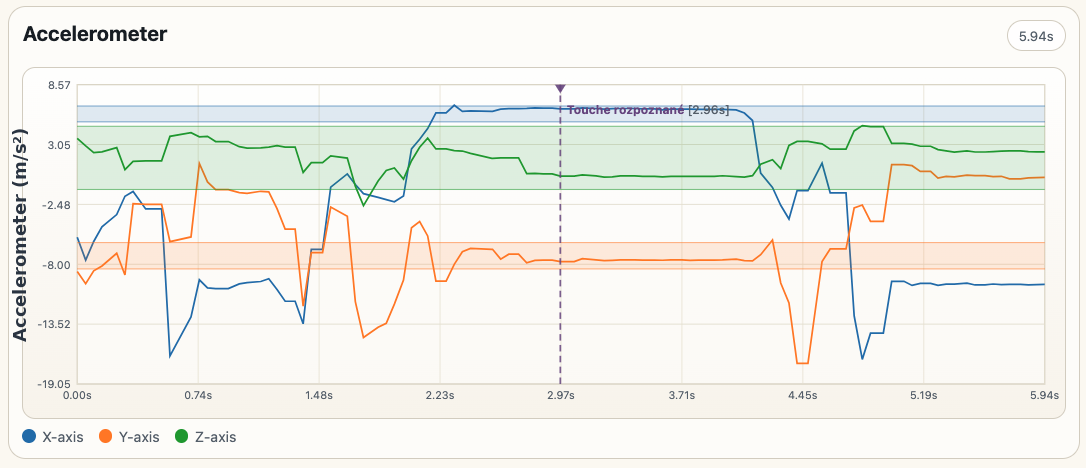
\includegraphics[width=0.9\textwidth]{img/gesture-flow/flow-gesto-touche.png}
  \caption{Priebeh akcelerometrických
    dát počas gesta \uv{TOUCHE}.}
  \label{fig:subgesture-touche}
\end{figure}

Na obrázku~\ref{fig:subgesture-touche} je zobrazený priebeh akcelerometrických
dát počas vykonania gesta \uv{TOUCHE}. Hodnoty osí sa po preložení ruky
cez hruď ustália v~rámci definovaných intervalov hodnôt.

\noindent
\textbf{Interval hodnôt:}

\begin{itemize}
  \item \colorbox{xaxis!20}{$\toucheAxMin \leq a_x \leq \toucheAxMax \;\text{m/s}^2$}
  \item \colorbox{yaxis!20}{$\toucheAyMin \leq a_y \leq \toucheAyMax \;\text{m/s}^2$}
  \item \colorbox{zaxis!20}{$\toucheAzMin \leq a_z \leq \toucheAzMax \;\text{m/s}^2$}
\end{itemize}
